\documentclass[spanish]{article}

\usepackage{mystyle}
\usepackage{myvars}
\usepackage{mylinearprogramming}



%-----------------------------

\begin{document}

	\maketitle % Insert title

	\thispagestyle{fancy} % All pages have headers and footers


%-----------------------------
%	ABSTRACT
%-----------------------------

	\begin{abstract}
		\noindent [TODO ]
	\end{abstract}

%-----------------------------
%	TEXT
%-----------------------------

	\section{Introducción}

		\paragraph{}
		[TODO ]

	\setcounter{section}{5}

	\section{Set-Covering Problem}
	\label{sec:e-6}

		\paragraph{}
		El problema de \emph{Set Covering} o \emph{Cubrimiento de Conjuntos} consiste en la asignación de un conjunto de recursos $n$ recursos $x_{j}$ cuyo uso tiene un coste de $c_{j}$ para cumplir $m$ necesidades. Las necesidades que cubre cada recurso se representan a través de $a_{ij}$. La modelización matemática de este problema se muestra en la ecuación \eqref{eq:set_covering}.

		\begin{eqfloat}
			\begin{equation}
				\begin{array}{ll@{}ll}
					\text{Minimizar}	& \displaystyle\sum\limits_{j=1}^{n} c_{j}	&	x_{j} &\\
					\text{sujeto a}		& \displaystyle\sum\limits_{j = 1}^n a_{ij}	&	x_{j} \geq 1,  &i=1 ,..., m\\
														&                                           &	x_{j} \in \{0,1\}, &j=1 ,..., n
				\end{array}
			\end{equation}
			\caption{Formulación de \emph{Set-Covering Problem}.}
			\label{eq:set_covering}
		\end{eqfloat}

		\paragraph{}
		[TODO describir heurísticas]

		\subsection{Ejercicio Nueva York}
		\label{sec:e-6.1}

			\paragraph{}
			En este caso, se ha propuesto resolver el problema de \emph{Cubrimiento de Conjuntos} sobre un conjunto de datos de entrada referidos a las distancias entre $30$ distritos de la ciudad de Nueva York. Se considera que un distrito ha sido cubierto si la distancia a un punto de servicio es menor o igual que un determinado valor $dc$ denominado distancia de cubrimiento. En este caso se ha resuelto para valores enteros comprendidos en el intervalo $[70, 120]$ mediante la estrategia \emph{Greedy} y la de \emph{Solución Óptima}. Los resultados obtenidos se muestran gráficamente en la figura \ref{fig:sol-6.1} y de manera tabular en la tabla \ref{table:sol-6.1}


			\begin{figure}[h]
				\begin{center}
					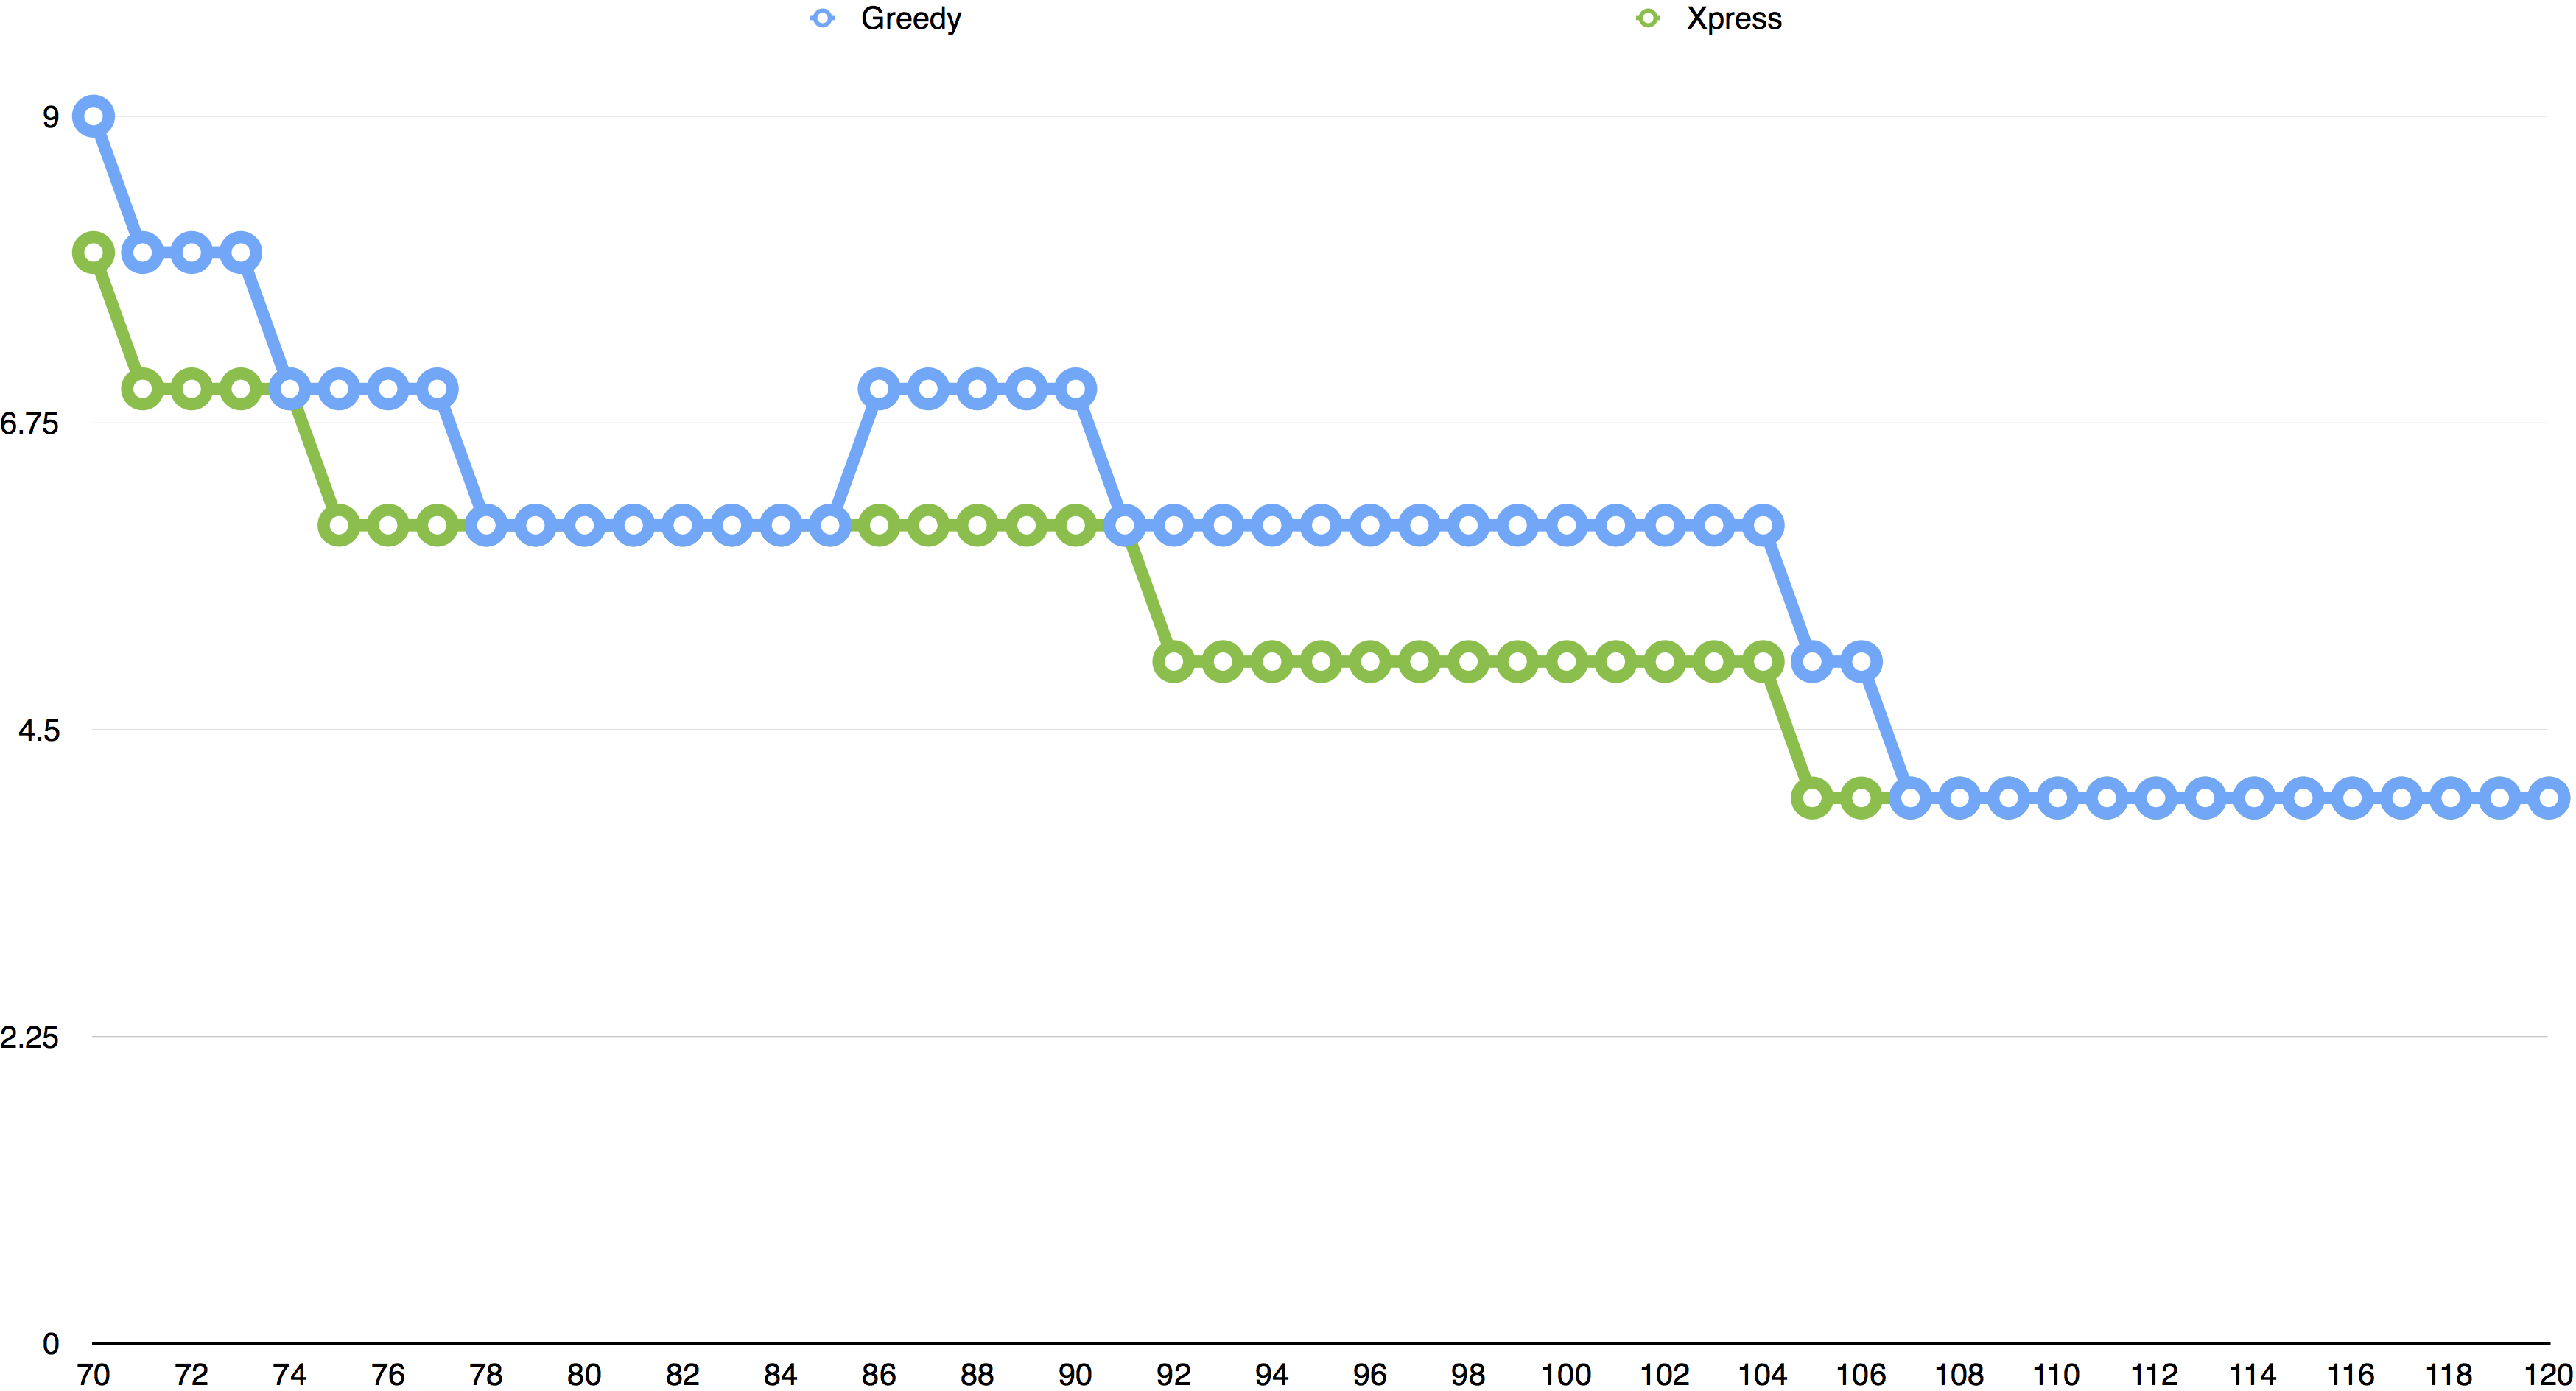
\includegraphics[width=0.8\textwidth]{tema-3-p6-1}
				\end{center}
				\caption{Resultados del problema de \emph{Set Covering} aplicado a los datos de los distritos de la ciudad de Nueva York}
				\label{fig:sol-6.1}
			\end{figure}


			\begin{table}[h]
				\begin{center}
					\csvautotabular{../results/csv/tema-3-p6-1.csv}
				\end{center}
				\caption{Resultados del problema de \emph{Set Covering} aplicado a los datos de los distritos de la ciudad de Nueva York}
				\label{table:sol-6.1}
			\end{table}

		\subsection{Ejercicio \emph{aint1}}
		\label{sec:e-6.2a}

			\paragraph{}
			En este caso, se ha propuesto resolver el problema de \emph{Cubrimiento de Conjuntos} sobre un conjunto de datos de entrada de tamaño relativamente elevado, con $m = 356$ puntos de demanda y $n=22$ puntos de servicio . Se considera que un distrito ha sido cubierto si la distancia a un punto de servicio es menor o igual que un determinado valor $dc$ denominado distancia de cubrimiento. En este caso se ha resuelto para valores enteros comprendidos en el intervalo $[250, 400]$ mediante la estrategia \emph{Greedy}, la estrategia \emph{Greedy Aleatorizada}(con parámetros $k=5$ y $n=100$)  y la de \emph{Solución Óptima}. Los resultados obtenidos se muestran gráficamente en la figura \ref{fig:sol-6.2a} y de manera tabular en las tablas \ref{table:sol-6.2a1}, \ref{table:sol-6.2a2} y \ref{table:sol-6.2a3}.

			\begin{figure}[h]
				\begin{center}
					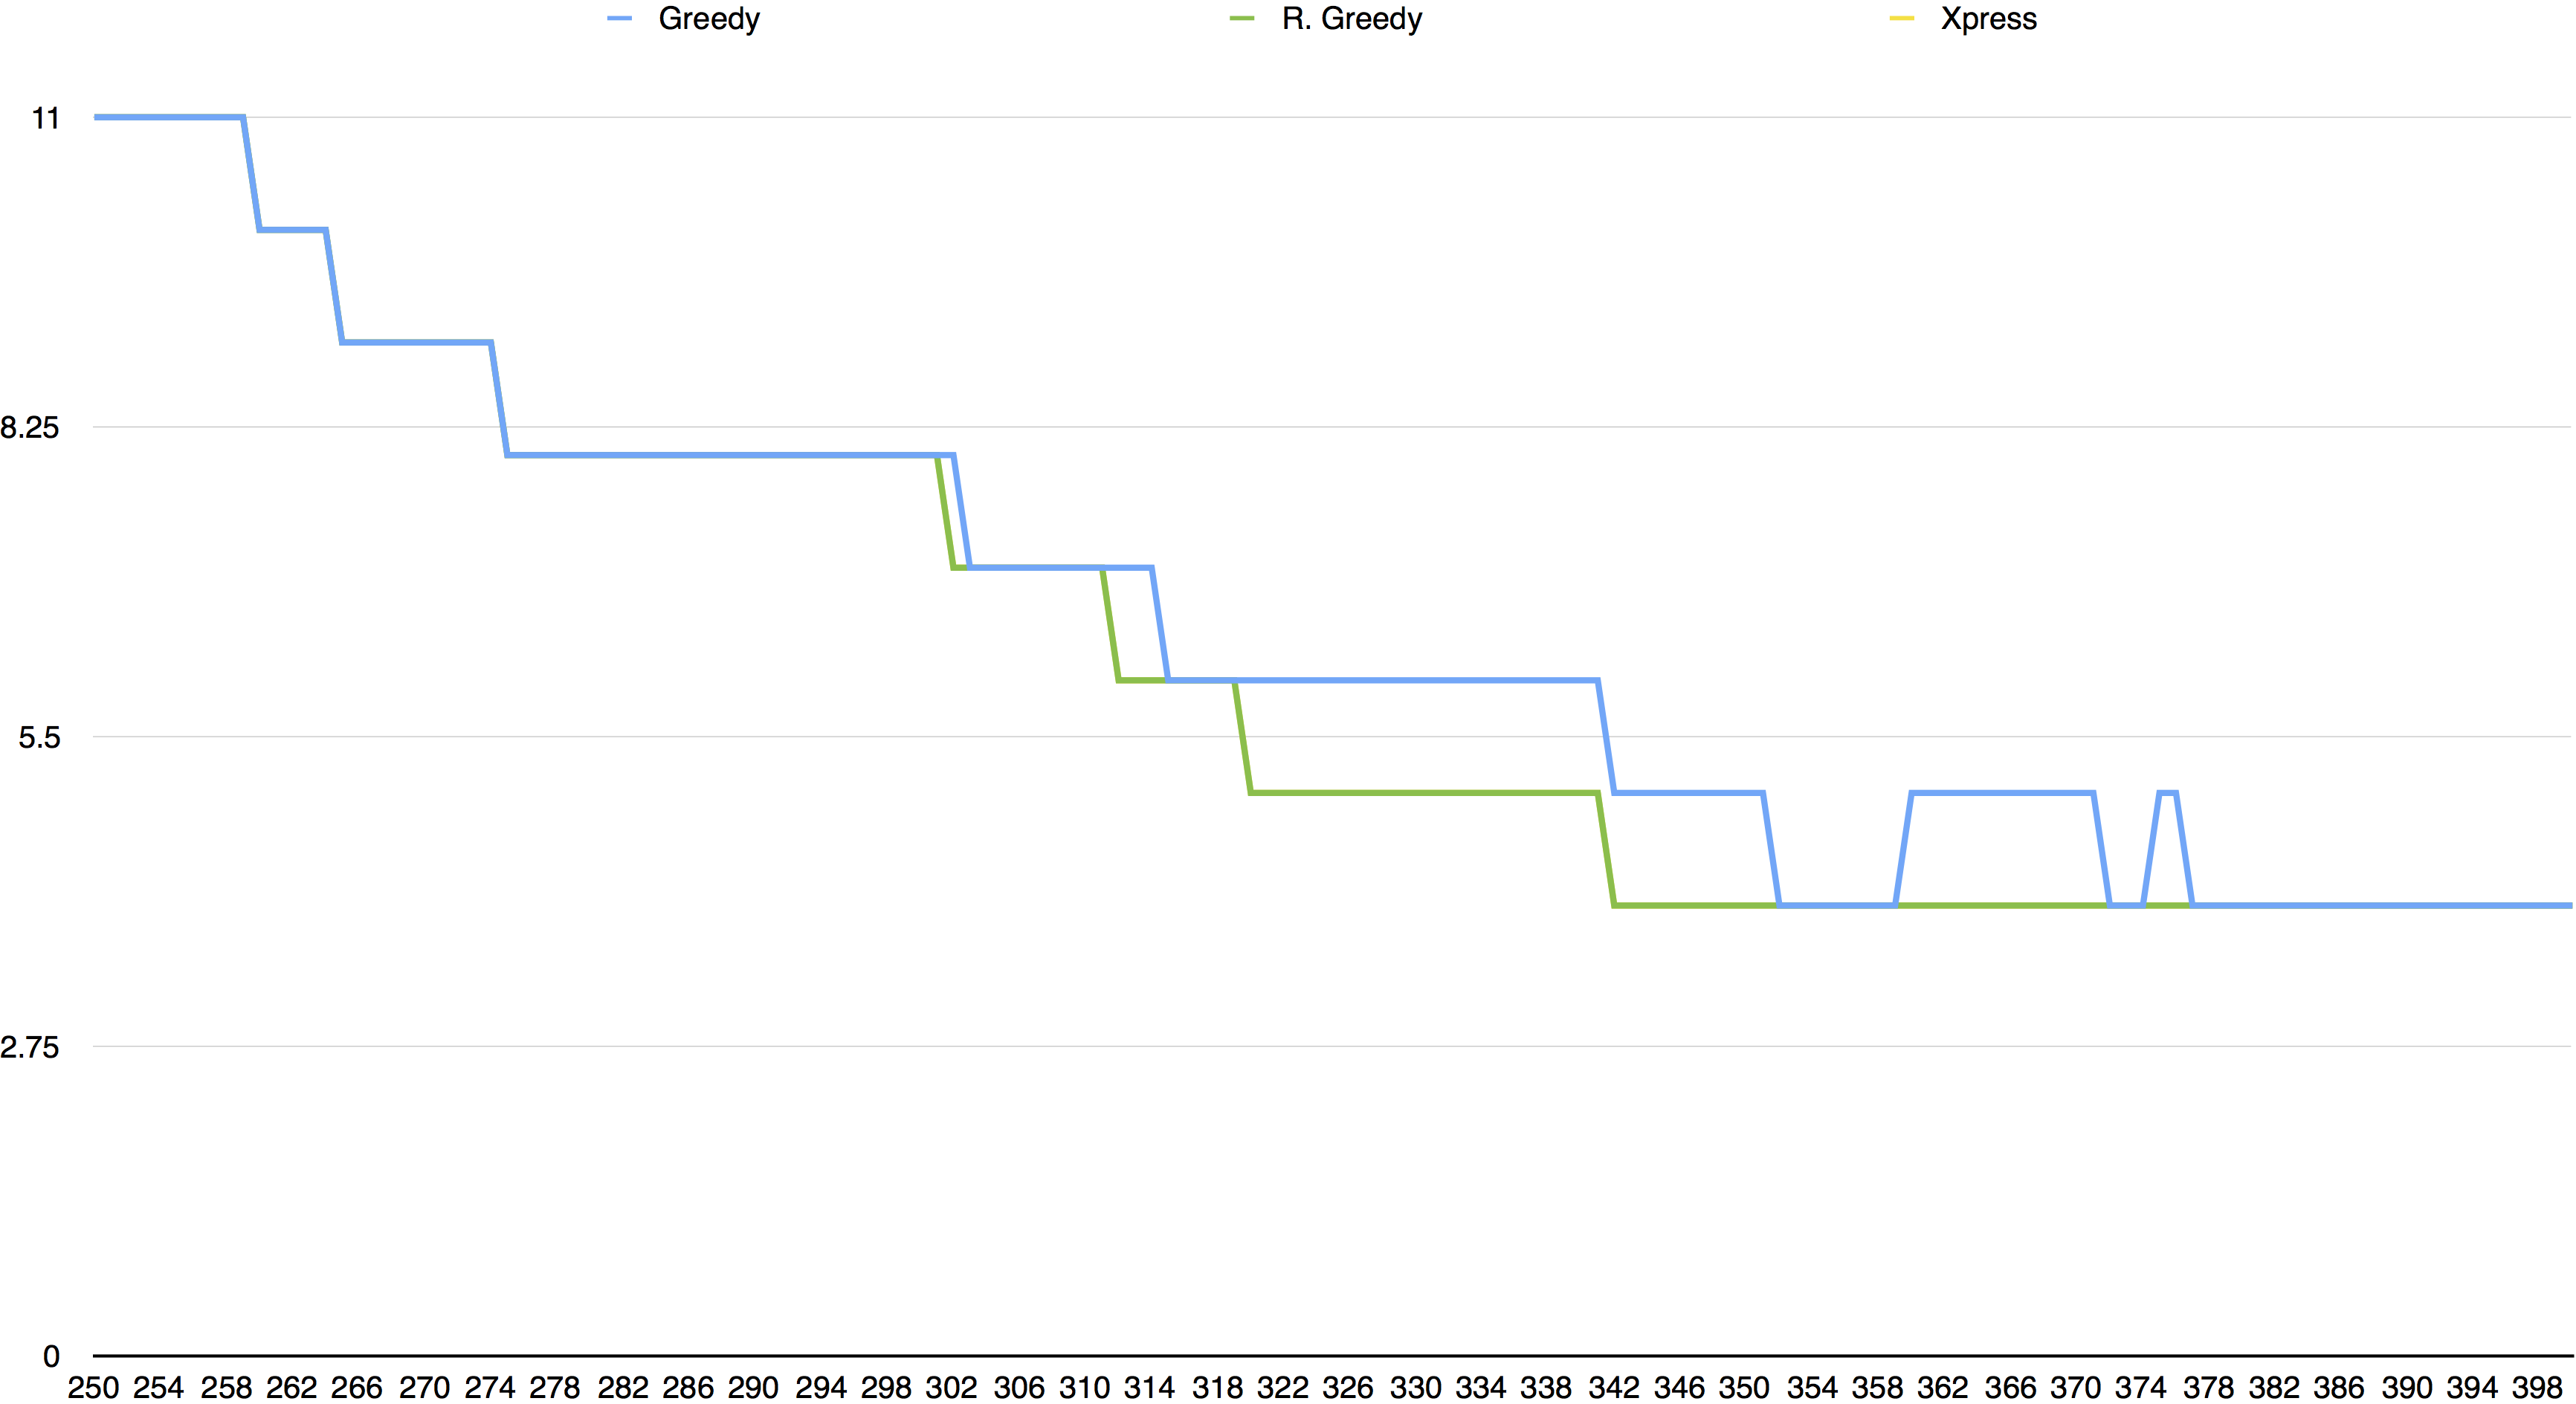
\includegraphics[width=0.8\textwidth]{tema-3-p6-2-a}
				\end{center}
				\caption{Resultados del problema de \emph{Set Covering} aplicado a los datos \emph{aint1}}
				\label{fig:sol-6.2a}
			\end{figure}

			\begin{table}[h]
				\begin{center}
					\csvautotabular{../results/csv/tema-3-p6-2-a-1.csv}
				\end{center}
				\caption{Resultados del problema de \emph{Set Covering} aplicado a los datos \emph{aint1}}
				\label{table:sol-6.2a1}
			\end{table}

			\begin{table}[h]
				\begin{center}
					\csvautotabular{../results/csv/tema-3-p6-2-a-2.csv}
				\end{center}
				\caption{Resultados del problema de \emph{Set Covering} aplicado a los datos \emph{aint1}}
				\label{table:sol-6.2a2}
			\end{table}

			\begin{table}[h]
				\begin{center}
					\csvautotabular{../results/csv/tema-3-p6-2-a-3.csv}
				\end{center}
				\caption{Resultados del problema de \emph{Set Covering} aplicado a los datos \emph{aint1}}
				\label{table:sol-6.2a3}
			\end{table}

		\subsection{Ejercicio \emph{aint5}}
		\label{sec:e-6.2b}

		\paragraph{}
		En este caso, se ha propuesto resolver el problema de \emph{Cubrimiento de Conjuntos} sobre un conjunto de datos de entrada de tamaño relativamente elevado, con $m = 328$ puntos de demanda y $n=19$ puntos de servicio . Se considera que un distrito ha sido cubierto si la distancia a un punto de servicio es menor o igual que un determinado valor $dc$ denominado distancia de cubrimiento. En este caso se ha resuelto para valores enteros comprendidos en el intervalo $[250, 400]$ mediante la estrategia \emph{Greedy}, la estrategia \emph{Greedy Aleatorizada}(con parámetros $k=5$ y $n=100$)  y la de \emph{Solución Óptima}. Los resultados obtenidos se muestran gráficamente en la figura \ref{fig:sol-6.2b} y de manera tabular en las tablas \ref{table:sol-6.2b1}, \ref{table:sol-6.2b2} y \ref{table:sol-6.2b3}.

			\begin{figure}[h]
				\begin{center}
					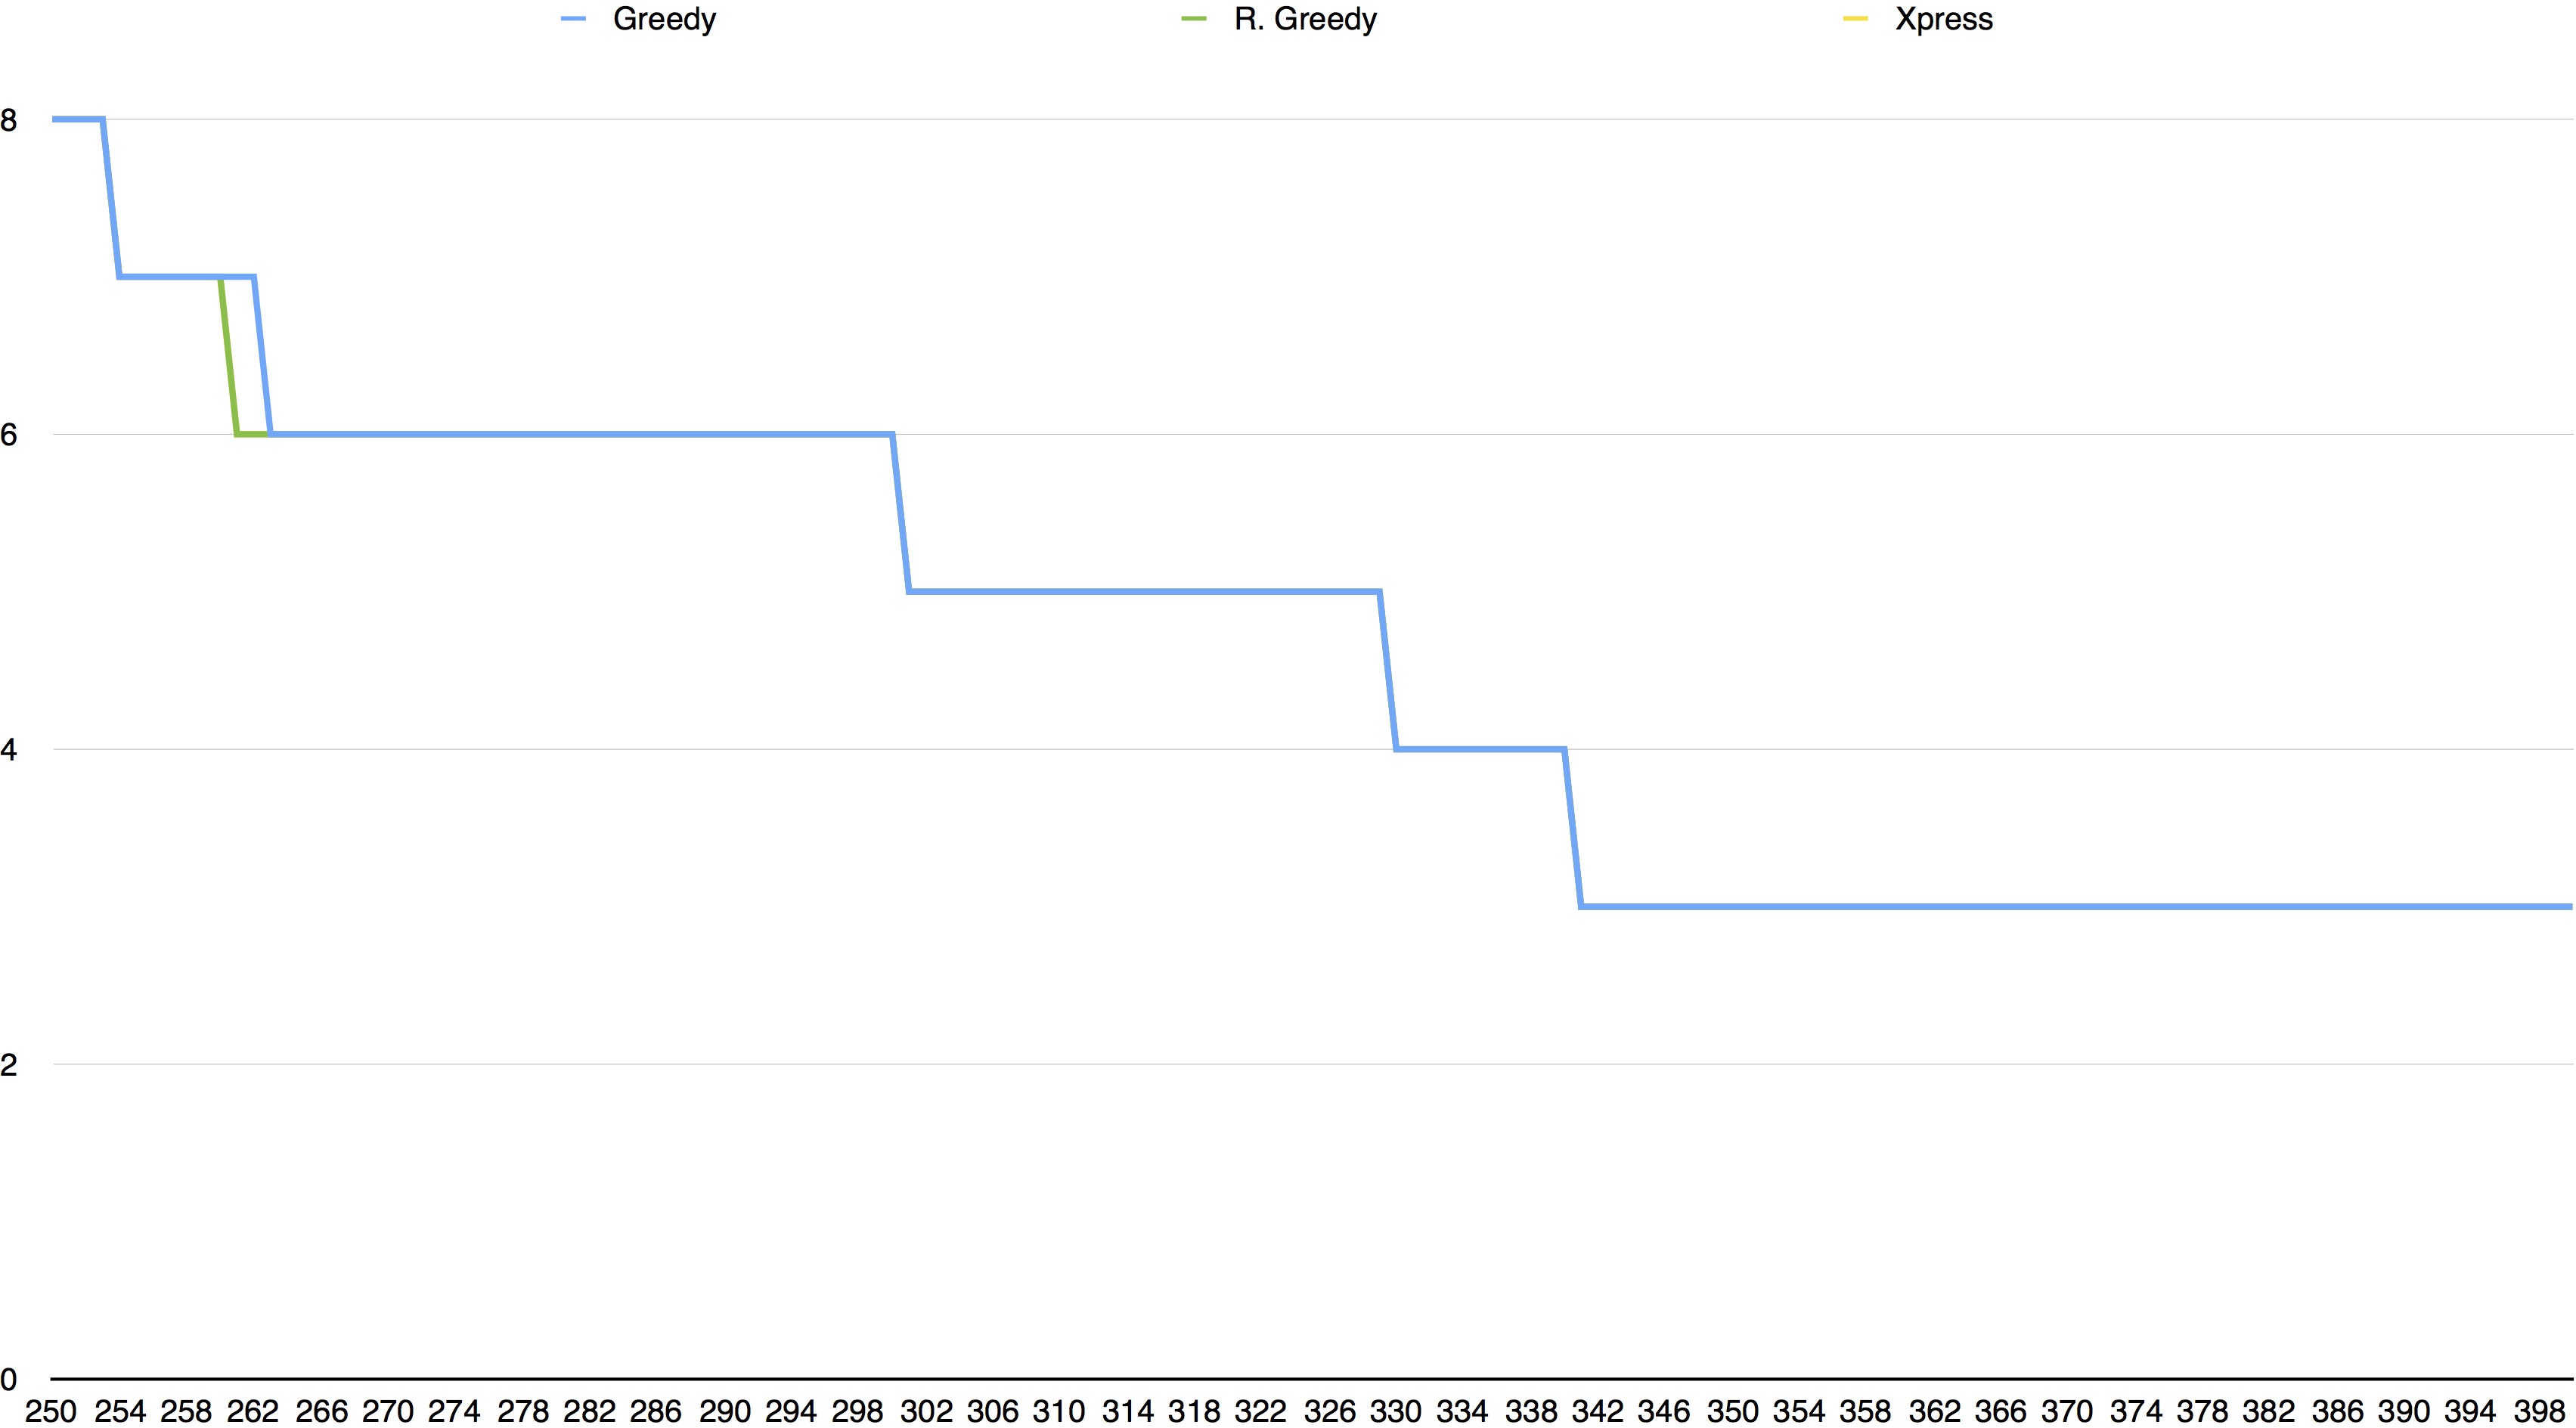
\includegraphics[width=0.8\textwidth]{tema-3-p6-2-b}
				\end{center}
				\caption{Resultados del problema de \emph{Set Covering} aplicado a los datos \emph{aint5}}
				\label{fig:sol-6.2b}
			\end{figure}

			\begin{table}[h]
				\begin{center}
					\csvautotabular{../results/csv/tema-3-p6-2-b-1.csv}
				\end{center}
				\caption{Resultados del problema de \emph{Set Covering} aplicado a los datos \emph{aint5}}
				\label{table:sol-6.2b1}
			\end{table}

			\begin{table}[h]
				\begin{center}
					\csvautotabular{../results/csv/tema-3-p6-2-b-2.csv}
				\end{center}
				\caption{Resultados del problema de \emph{Set Covering} aplicado a los datos \emph{aint5}}
				\label{table:sol-6.2b2}
			\end{table}

			\begin{table}[h]
				\begin{center}
					\csvautotabular{../results/csv/tema-3-p6-2-b-3.csv}
				\end{center}
				\caption{Resultados del problema de \emph{Set Covering} aplicado a los datos \emph{aint5}}
				\label{table:sol-6.2b3}
			\end{table}

	\section{Max-Covering Problem}
	\label{sec:e-7}

		\paragraph{}
		En esta sección se trata el \emph{problema de cubrimiento máximo} o \emph{max covering problem}. El problema consiste en lo siguiente: Sea $m$ el número de puntos de demandas y $n$ el de puntos de servicio. El objetivo se trata de maximizar el beneficio $h_i$ obtenido de cubrir el í-esimo punto de demanda. Para modelizar dicho cubrimiento se utiliza la variable binaria $z_i$. Para representar los puntos de servicio utilizados se utiliza la variable de tipo binario $x_j$. La motivación del problema consiste en encontrar el conjunto de variables $x_j$ con cardinalidad máxima denominada por $p$ y prefijada previamente, que máximize la ganancia debida al cubrimiento de los puntos de servicio $z_i$. El modelo formal se muestra en la ecuación \eqref{eq:max_covering}.

		\begin{eqfloat}
			\begin{equation}
				\begin{array}{ll@{}ll}
					\text{Maximizar}
						& \displaystyle\sum\limits_{i = 1}^{m} h_{i} & z_{i} 			&							\\
					\text{sujeto a}
						& \displaystyle\sum\limits_{j \in N_i}& x_{j} \geq z_i,		&i=1 ,..., m	\\
						& \displaystyle\sum\limits_{j = 1}^n 	& x_{j} \leq p,  		& 						\\
						&                                     &	x_{j} \in \{0,1\},&j=1 ,..., n 	\\
						&                                     &	z_{i} \in \{0,1\},&i=1 ,..., m  \\
				\end{array}
			\end{equation}
			\caption{Formulación de \emph{Max-Covering Problem}.}
			\label{eq:max_covering}
		\end{eqfloat}

		\paragraph{}
		[TODO describir heurísticas]


		\subsection{Ejercicio \emph{aint1}}
		\label{sec:e-7a}

			\paragraph{}
			En este caso, se ha propuesto resolver el problema de \emph{Cubrimiento Máximo} sobre un conjunto de datos de entrada de tamaño relativamente elevado, con $m = 356$ puntos de demanda y $n=22$ puntos de servicio . Se considera que un distrito ha sido cubierto si la distancia a un punto de servicio es menor o igual que un determinado valor $dc$ denominado distancia de cubrimiento. En este caso se ha resuelto para $dc = 200$ y un número de puntos de servicios restringido a $p = [1,6]$, mediante la estrategia \emph{Greedy}, la estrategia \emph{Greedy Aleatorizada}(con parámetros $k=5$ y $n=100$) y la de \emph{Solución Óptima}. Los resultados obtenidos se muestran gráficamente en la figura \ref{fig:sol-7a} y de manera tabular en las tablas \ref{table:sol-7a}.

			\begin{figure}[h]
				\begin{center}
					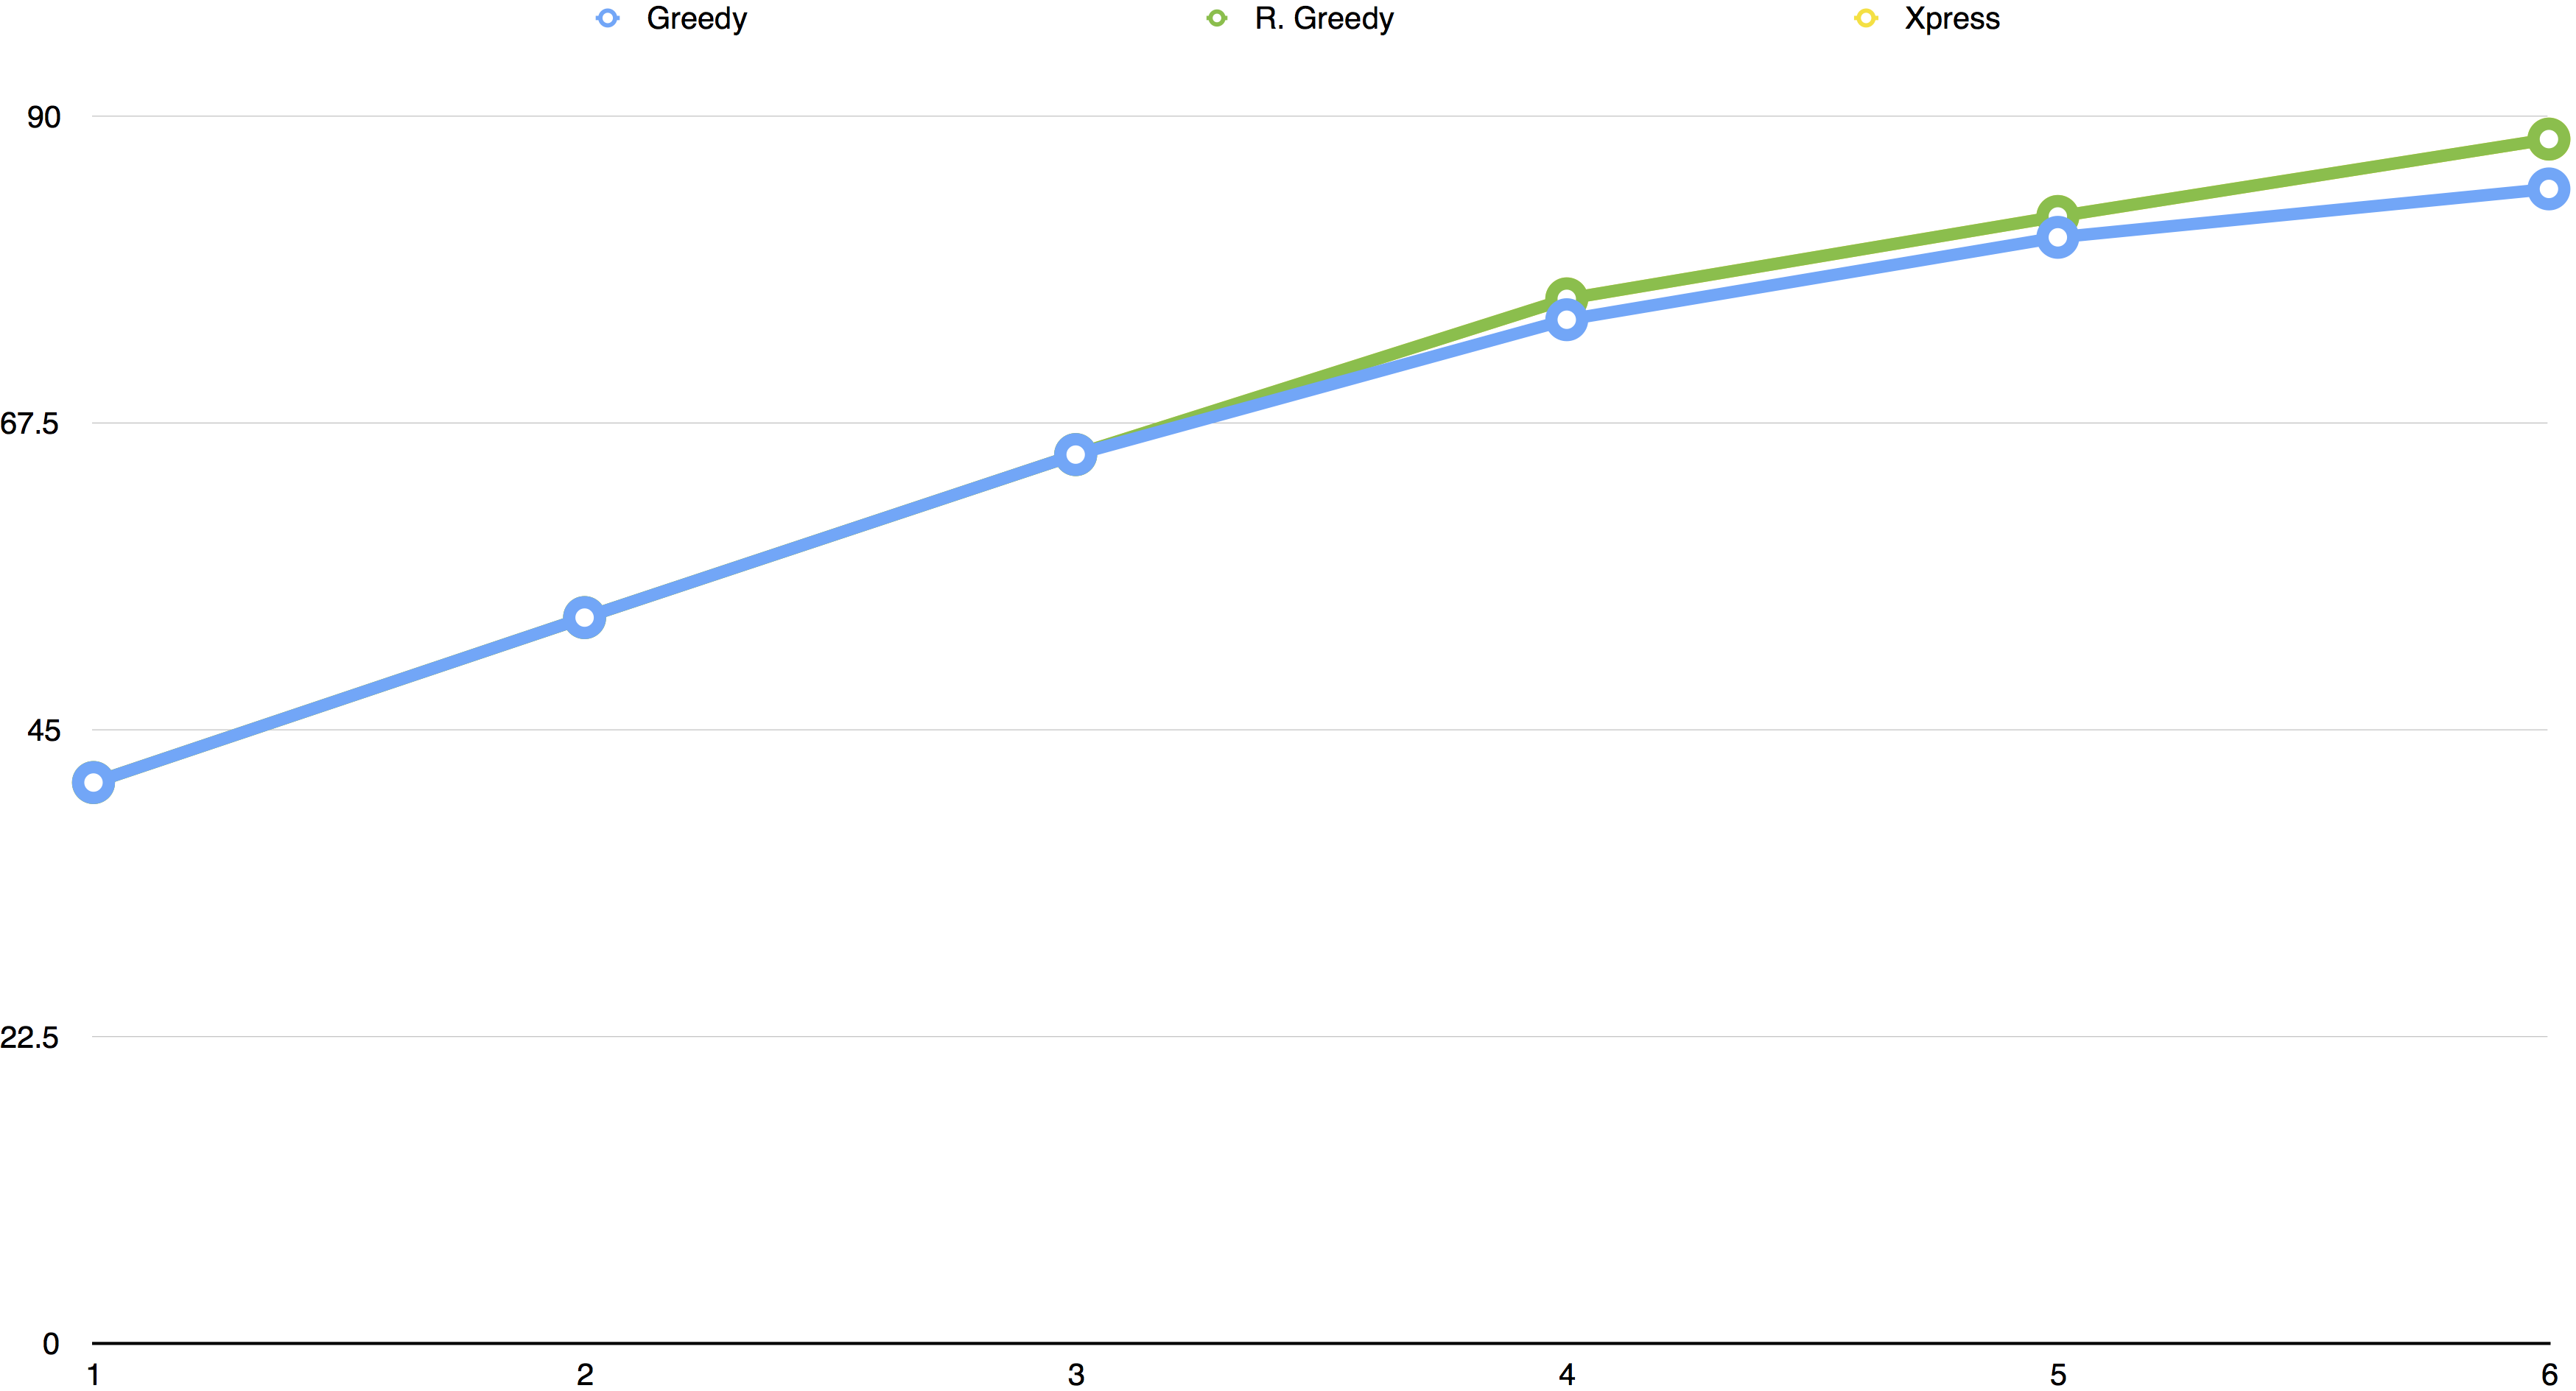
\includegraphics[width=0.8\textwidth]{tema-3-p7-a}
				\end{center}
				\caption{Resultados del problema de \emph{Max Covering} aplicado a los datos \emph{aint1}}
				\label{fig:sol-7a}
			\end{figure}

			\begin{table}[h]
				\begin{center}
					\csvautotabular{../results/csv/tema-3-p7-a.csv}
				\end{center}
				\caption{Resultados del problema de \emph{Max Covering} aplicado a los datos \emph{aint1}}
				\label{table:sol-7a}
			\end{table}

		\subsection{Ejercicio \emph{aint5}}
		\label{sec:e-7b}

			\paragraph{}
			En este caso, se ha propuesto resolver el problema de \emph{Cubrimiento Máximo} sobre un conjunto de datos de entrada de tamaño relativamente elevado, con $m = 328$ puntos de demanda y $n=19$ puntos de servicio . Se considera que un distrito ha sido cubierto si la distancia a un punto de servicio es menor o igual que un determinado valor $dc$ denominado distancia de cubrimiento. En este caso se ha resuelto para $dc = 200$ y un número de puntos de servicios restringido a $p = [1,6]$, mediante la estrategia \emph{Greedy}, la estrategia \emph{Greedy Aleatorizada}(con parámetros $k=5$ y $n=100$) y la de \emph{Solución Óptima}. Los resultados obtenidos se muestran gráficamente en la figura \ref{fig:sol-7b} y de manera tabular en las tablas \ref{table:sol-7b}.

			\begin{figure}[h]
				\begin{center}
					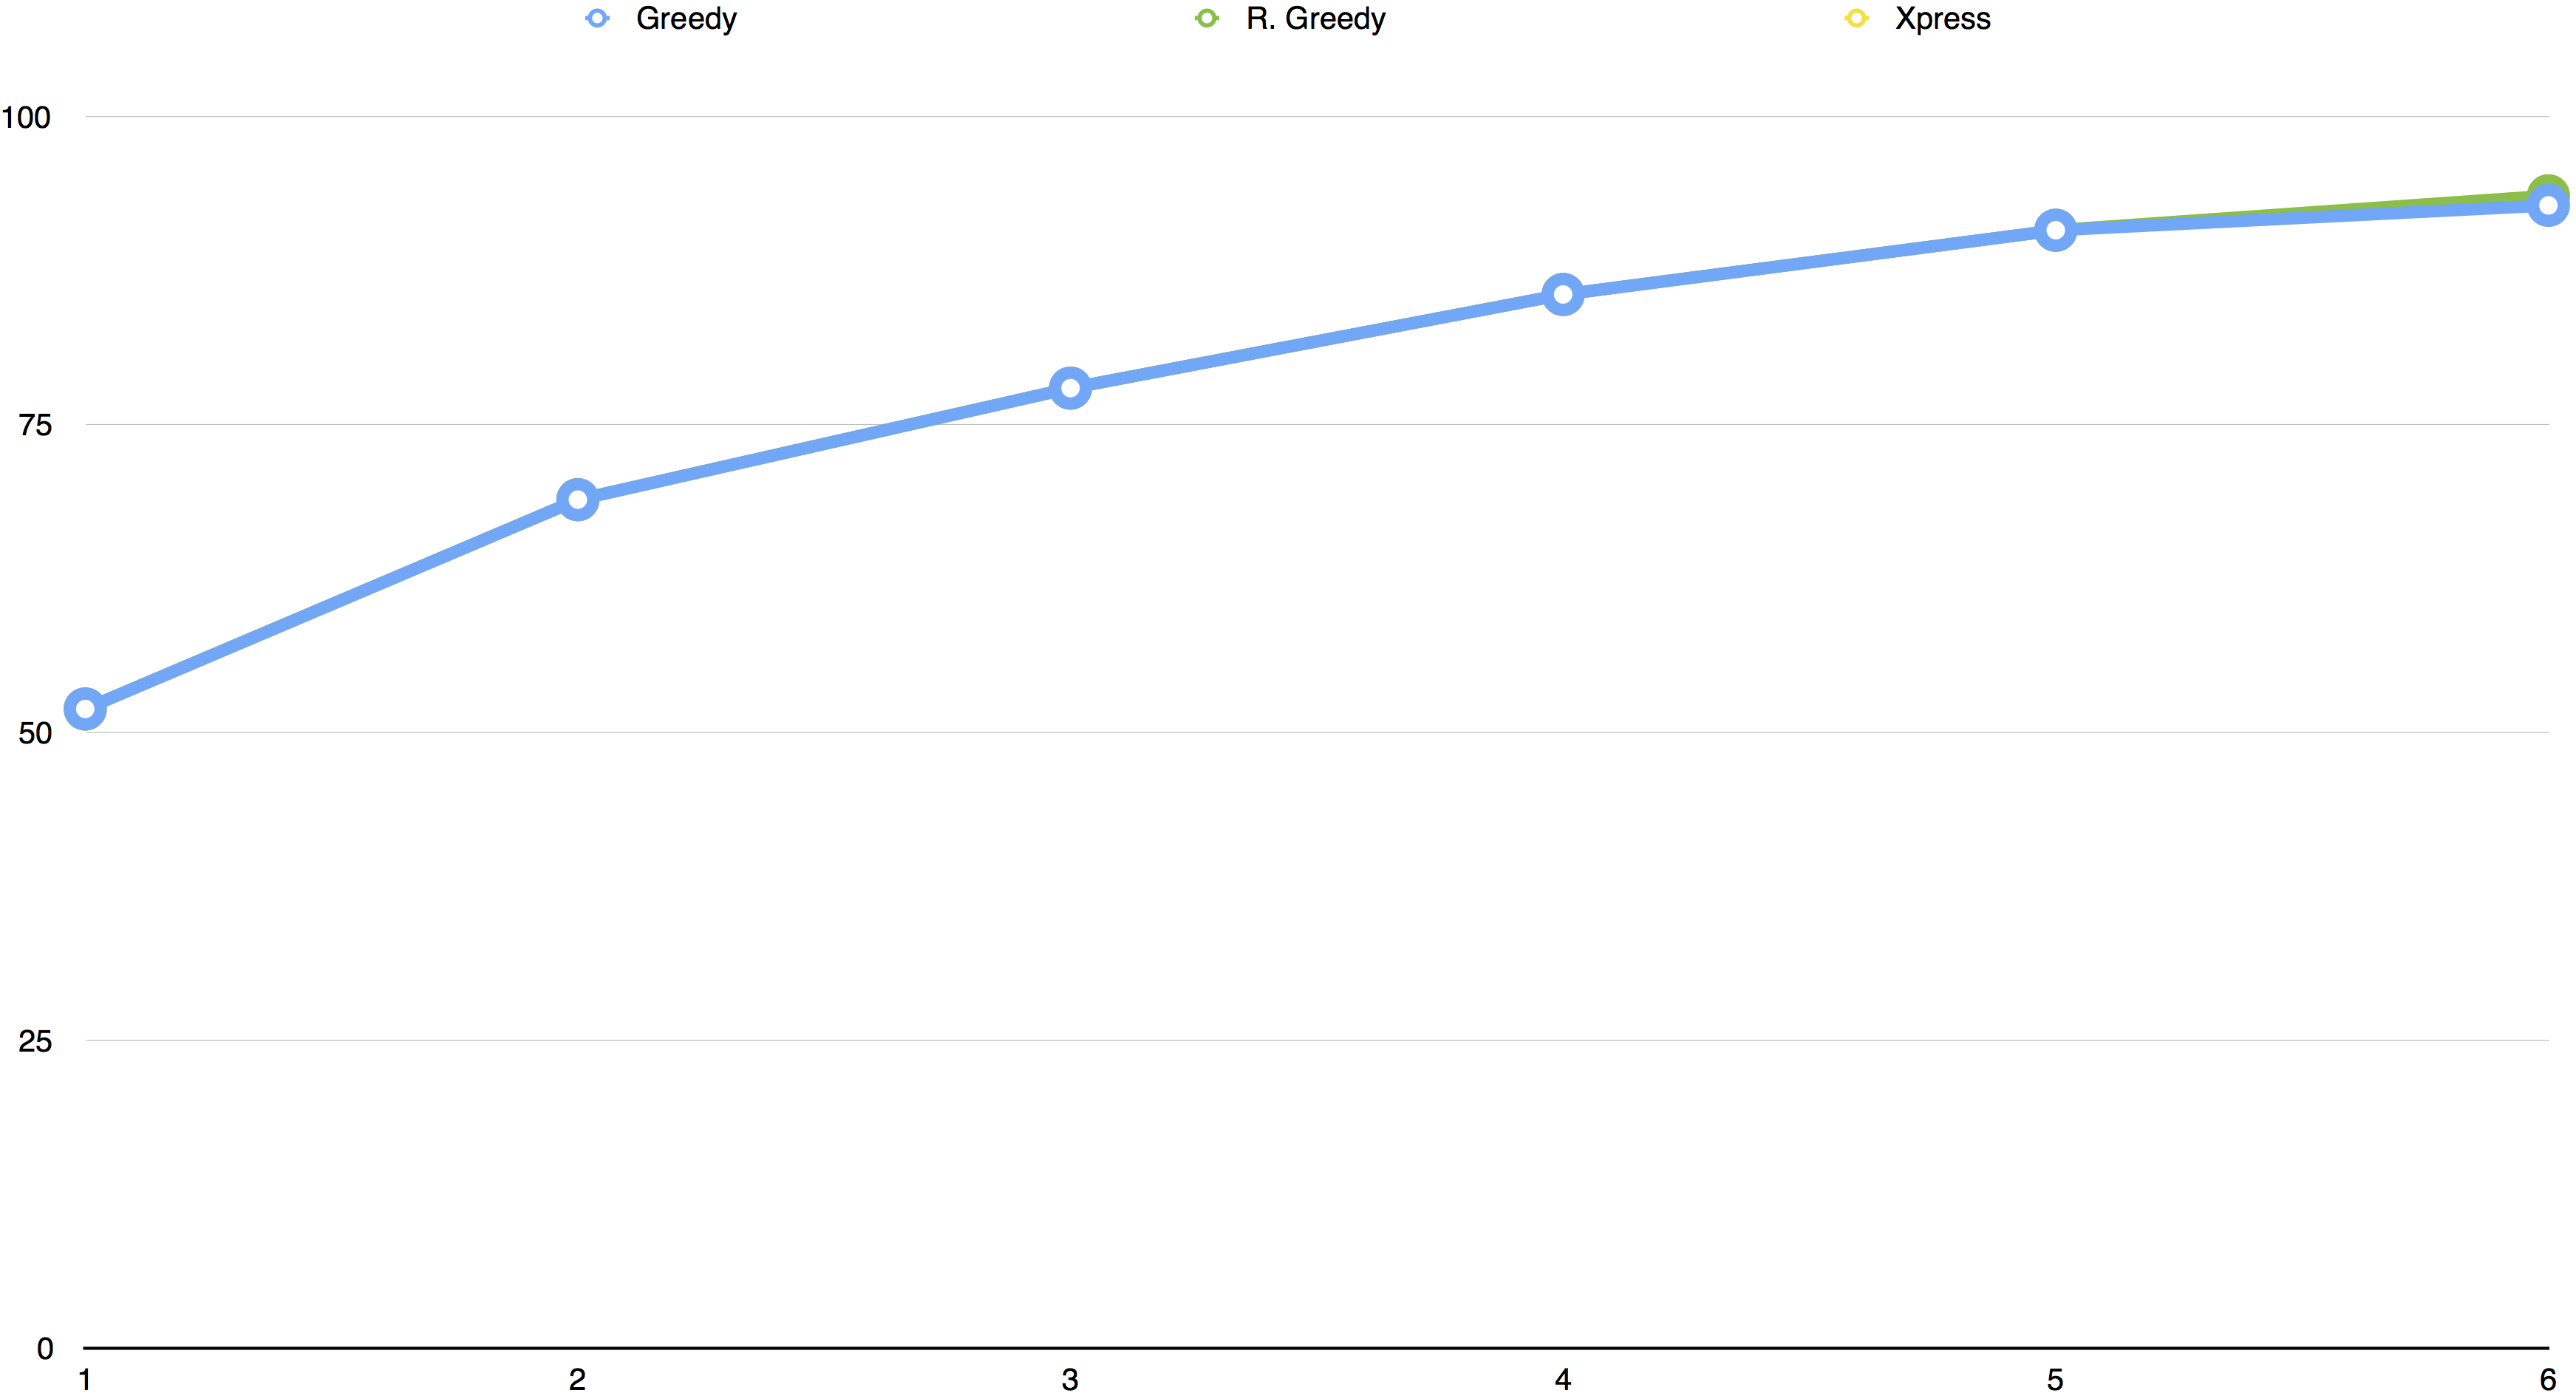
\includegraphics[width=0.8\textwidth]{tema-3-p7-b}
				\end{center}
				\caption{Resultados del problema de \emph{Max Covering} aplicado a los datos \emph{aint5}}
				\label{fig:sol-7b}
			\end{figure}

			\begin{table}[h]
				\begin{center}
					\csvautotabular{../results/csv/tema-3-p7-b.csv}
				\end{center}
				\caption{Resultados del problema de \emph{Max Covering} aplicado a los datos \emph{aint5}}
				\label{table:sol-7b}
			\end{table}


	\section{P-Median Problem}
	\label{sec:e-8}

		\paragraph{}
		En el caso del problema de la p-mediana, modelizado matemáticamente en la ecuación \ref{eq:p_median}, el objetivo es minimizar la distancia global de cada uno de los $p$ puntos de servicio abiertos al conjunto globla de puntos de demanda, de manera que los $j$ puntos de servicio abierto mantengan la menor distancia en promedio a los $i$ puntos de demanda.

		\paragraph{}
		En este problema, al igual que en los anteriores, se utiliza un vector de demanda denominado $h$, que en la componente $h_{i}$ almacena la demanda necesaria por el punto de demanda $i$. También existe una matriz de distancias de $d$, que en la posición $d_{ij}$ recoge la distancia del punto de demanda $i$ al punto de servicio $j$.

		\paragraph{}
		Para resolver este problema, además de las variables de decisión $x_j$ utilizadas en casos anteriores, que represntan que el punto de servicio $j$ está activo, se añaden las variables $y_ij$, que representan que el punto de demanda $i$ es servido por el punto de servicio $j$, lo que conlleva que en esta modelización cada punto de demanda sea servido únicamente por un único servicio.

		\begin{eqfloat}
			\begin{equation}
				\begin{array}{ll@{}ll}
					\text{Minimizar}
						& \displaystyle\sum\limits_{i = 1}^m
							\displaystyle\sum\limits_{j = 1}^n	& h_i d_{ij} y_{ij}	&							\\
					\text{sujeto a}
						& \displaystyle\sum\limits_{j = 1}^n 	& y_{ij} = 1,		& i = 1,..., m	\\
						& 																	 	& y_{ij} \leq x_{j},  		& i=1 ,..., m,j=1 ,..., n  \\
						& \displaystyle\sum\limits_{j = 1}^n 	& x_{j} = p,  		& 						\\
						&                                     &	x_{j} \in \{0,1\},&j=1 ,..., n 	\\
						&                                     &	y_{ij} \in \{0,1\},&i=1 ,..., m, j=1 ,..., n  \\
				\end{array}
			\end{equation}
			\caption{Formulación de \emph{P-Median Problem}.}
      \label{eq:p_median}
    \end{eqfloat}

		\paragraph{}
		[TODO describir heurísticas]

		\subsection{Ejercicio \emph{coordenadas\_15}}
		\label{sec:e-8a}

			\paragraph{}
			Este ejercicio tiene como novedad respecto de los anteriores la siguiente cateracterística: En este caso los datos de entrada no se presentan a partir de la matriz de distancias, tal y como sucedia en el resto, sino que se suministran las coordenadas $x$ e $y$ de cada localización. Esto hace que el problema permita una mayor versatilidad en el sentido de calcular un mayor número de resultados, pero a la vez añade la complicación de requerir el cálculo de las distancias entre puntos.

			\paragraph{}
			Para la tarea de calcular las distancias se ha utilizado la \emph{distancia euclidea} para espacios de 2 dimensiones $(x,y)$, que se define matemáticamente como $d(p, q) = \sqrt{(p_x - q_x)^2 + (p_y - q_y)^2}$. Por lo tanto, para la modelización del problema de la p-mediana, es necesario calcular dicha medida para todas las posibles combinaciones de localizaciones, de tal manera que la matriz $d$ sea construida siguiendo la expresión $d_{ij} = d(l_i, l_j)$ donde $l_i$ y $l_j$ representan las coordenadas de las localizaciones $i$ y $j$ respectivamente.


			\paragraph{}
			En esta sección se resuelve el problema de la \emph{P Mediana} mediante la estrategia \emph{Greedy}, la estrategia de \emph{Búsqueda Local} y la de \emph{Solución Óptima}. El conjunto de datos está compuesto por $n = m = 15$ poblaciones, para las cuales se pide resolver el problema para $p = [1,10] \in N$. Dichos resultados se muestran graficamente en la figura \ref{fig:sol-8a} y de manera tabular en la tabla \ref{table:sol-8a}. Además, se proporciona la solución gráfica en la figura \ref{fig:sol-8a-graph}.

			\begin{figure}[h]
				\begin{center}
					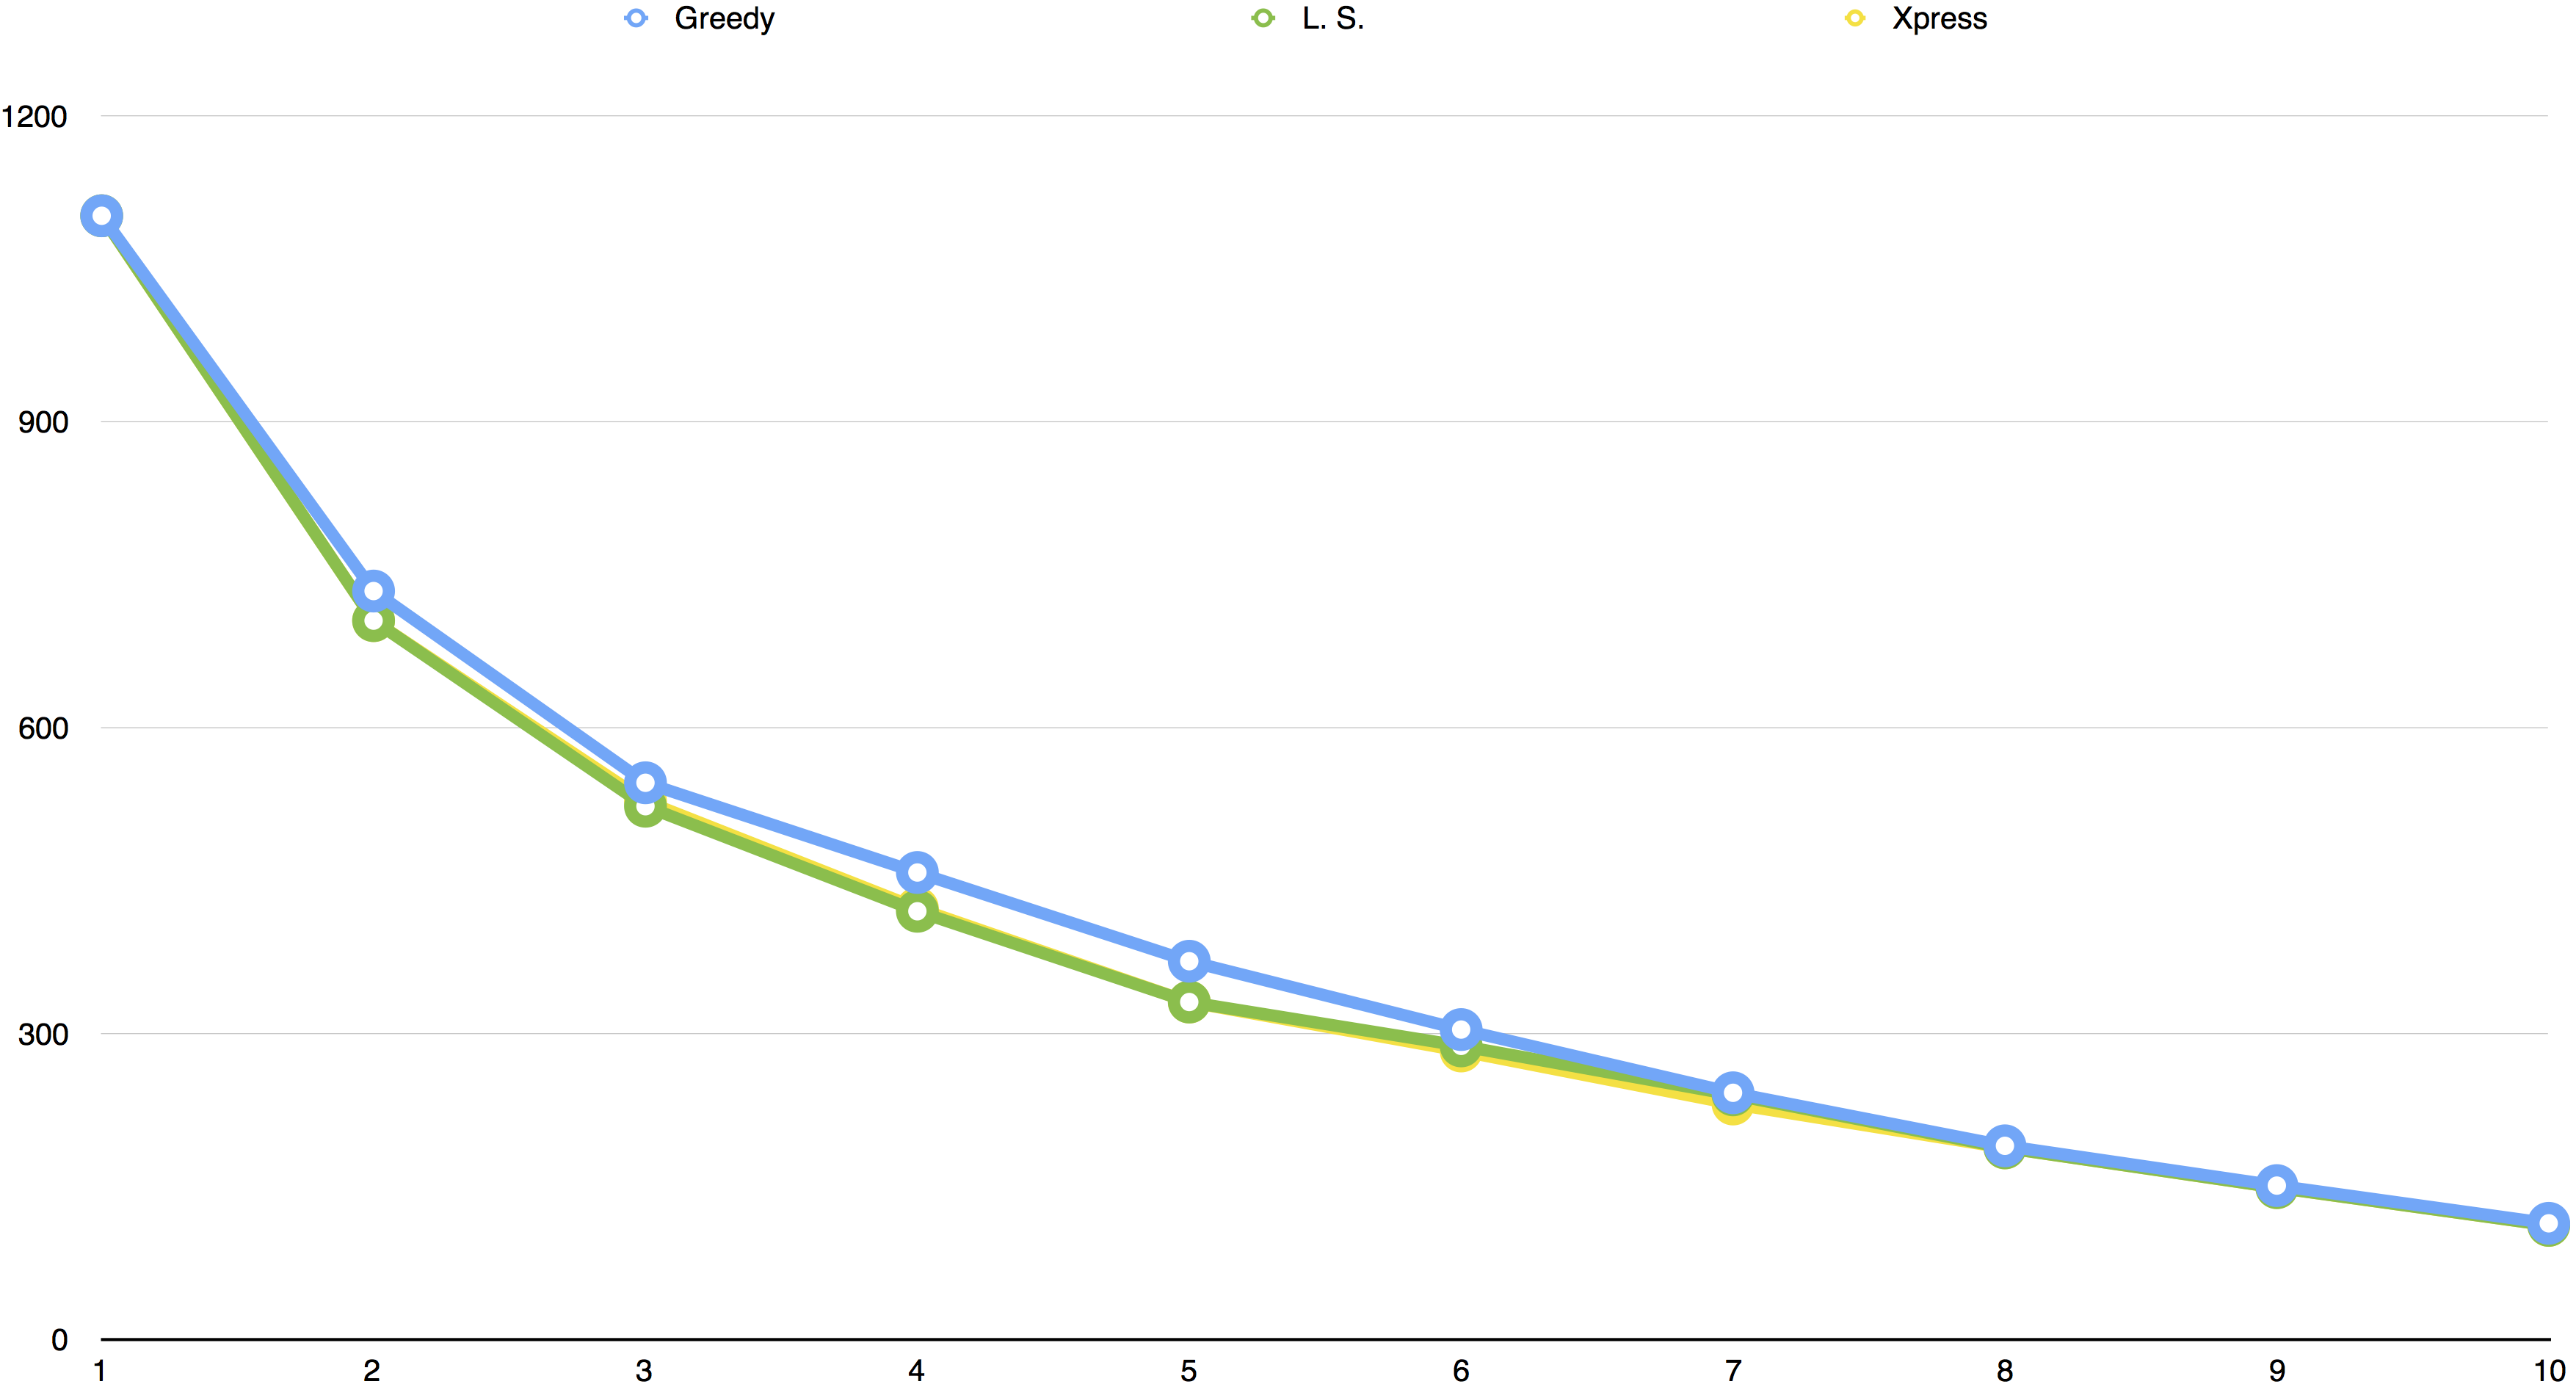
\includegraphics[width=0.8\textwidth]{tema-3-p8-a}
				\end{center}
				\caption{Resultados del problema \emph{P-Median} aplicado a los datos de \emph{15 poblaciones}}
				\label{fig:sol-8a}
			\end{figure}

			\begin{figure}[h]
				\begin{center}
					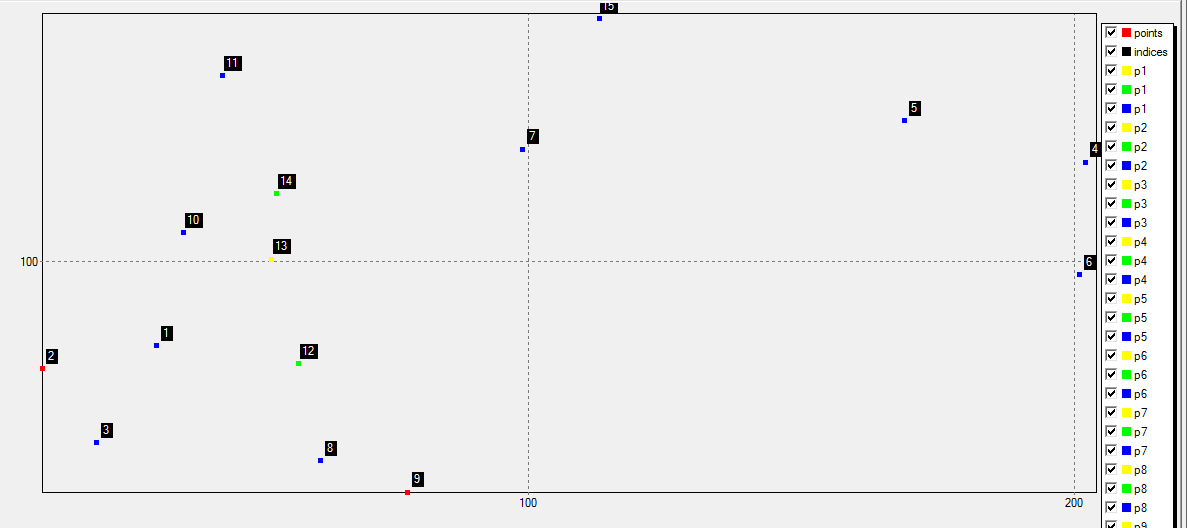
\includegraphics[width=0.8\textwidth]{tema-3-p8-a-graph}
				\end{center}
				\caption{Representación gráfica del problema \emph{P-Median} aplicado a los datos de \emph{15 poblaciones}}
				\label{fig:sol-8a-graph}
			\end{figure}

			\begin{table}[h]
				\begin{center}
					\caption{Resultados del problema \emph{P-Median} aplicado a los datos de \emph{15 poblaciones}}
				\end{center}
				\caption{[TODO ]}
				\label{table:sol-8a}
			\end{table}


		\subsection{Ejercicio \emph{coordenadas\_30}}
		\label{sec:e-8b}

			\paragraph{}
			En esta sección se resuelve el problema de la \emph{P Mediana} mediante la estrategia \emph{Greedy}, la estrategia de \emph{Búsqueda Local} y la de \emph{Solución Óptima}. El conjunto de datos está compuesto por $n = m = 30$ poblaciones, para las cuales se pide resolver el problema para $p = [1,10] \in N$. Dichos resultados se muestran graficamente en la figura \ref{fig:sol-8b} y de manera tabular en la tabla \ref{table:sol-8b}. Además, se proporciona la solución gráfica en la figura \ref{fig:sol-8b-graph}.


			\begin{figure}[h]
				\begin{center}
					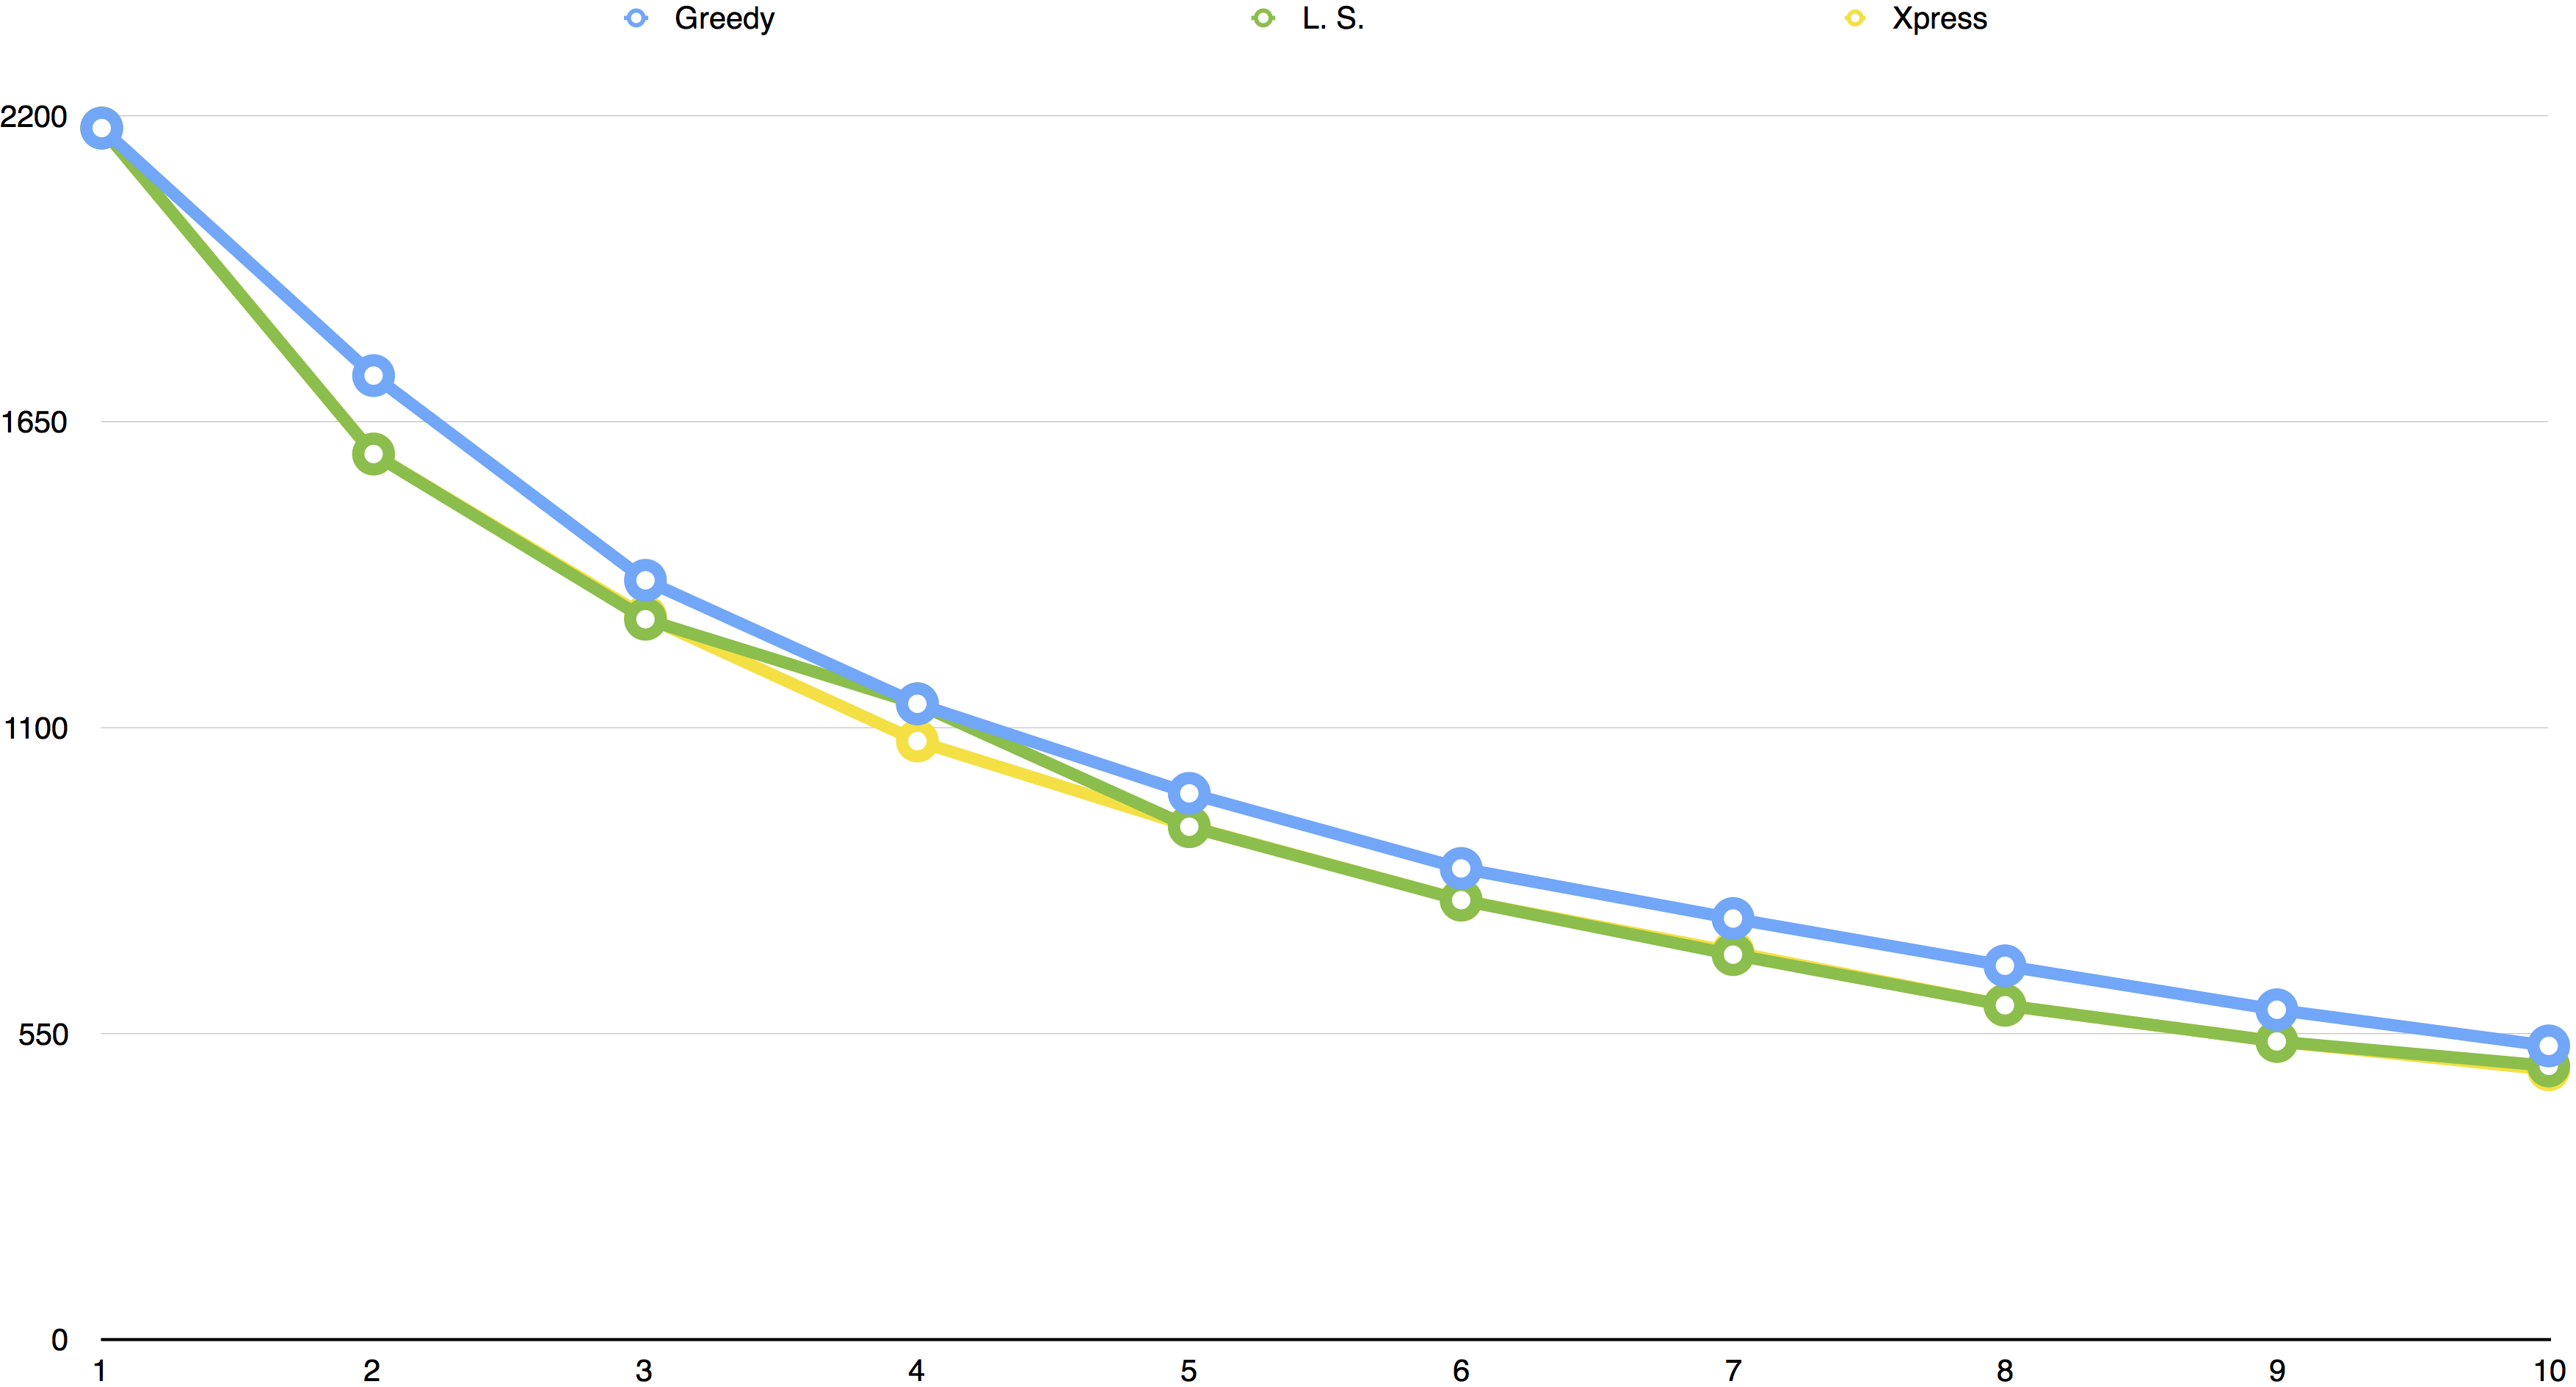
\includegraphics[width=0.8\textwidth]{tema-3-p8-b}
				\end{center}
				\caption{Resultados del problema \emph{P-Median} aplicado a los datos de \emph{30 poblaciones}}
				\label{fig:sol-8b}
			\end{figure}

			\begin{figure}[h]
				\begin{center}
					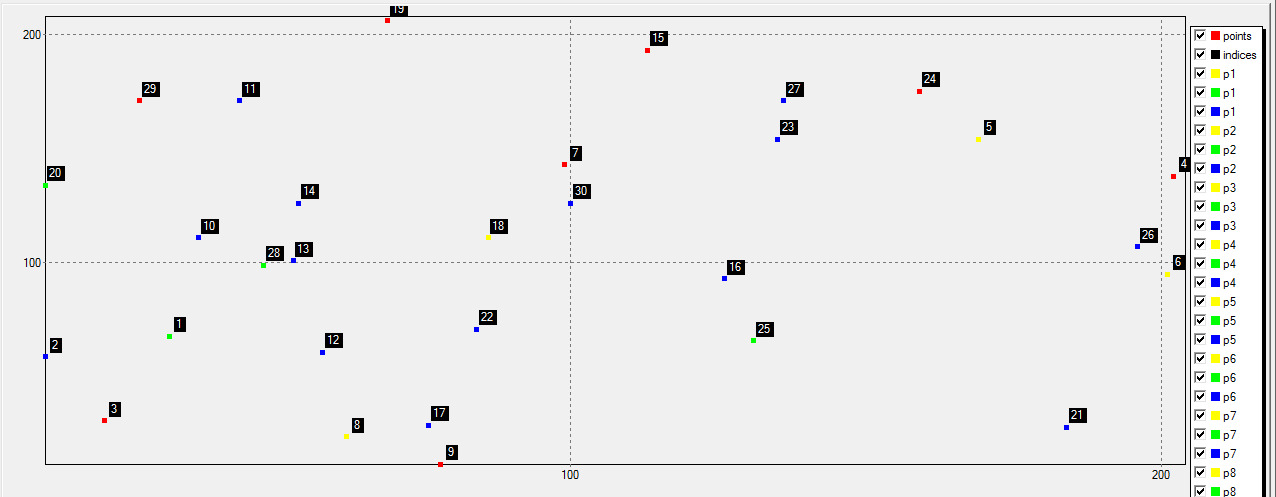
\includegraphics[width=0.8\textwidth]{tema-3-p8-b-graph}
				\end{center}
				\caption{Representación gráfica del problema \emph{P-Median} aplicado a los datos de \emph{30 poblaciones}}
				\label{fig:sol-8b-graph}
			\end{figure}

			\begin{table}[h]
				\begin{center}
					\csvautotabular{../results/csv/tema-3-p8-b.csv}
				\end{center}
				\caption{Resultados del problema \emph{P-Median} aplicado a los datos de \emph{30 poblaciones}}
				\label{table:sol-8b}
			\end{table}

		\subsection{Ejercicio \emph{coordenadas\_100}}
		\label{sec:e-8c}

			\paragraph{}
			En esta sección se resuelve el problema de la \emph{P Mediana} mediante la estrategia \emph{Greedy}, la estrategia de \emph{Búsqueda Local} y la de \emph{Solución Óptima}. El conjunto de datos está compuesto por $n = m = 100$ poblaciones, para las cuales se pide resolver el problema para $p = [1,10] \in N$. Dichos resultados se muestran graficamente en la figura \ref{fig:sol-8c} y de manera tabular en la tabla \ref{table:sol-8c}. Además, se proporciona la solución gráfica en la figura \ref{fig:sol-8c-graph}.


			\begin{figure}[h]
				\begin{center}
					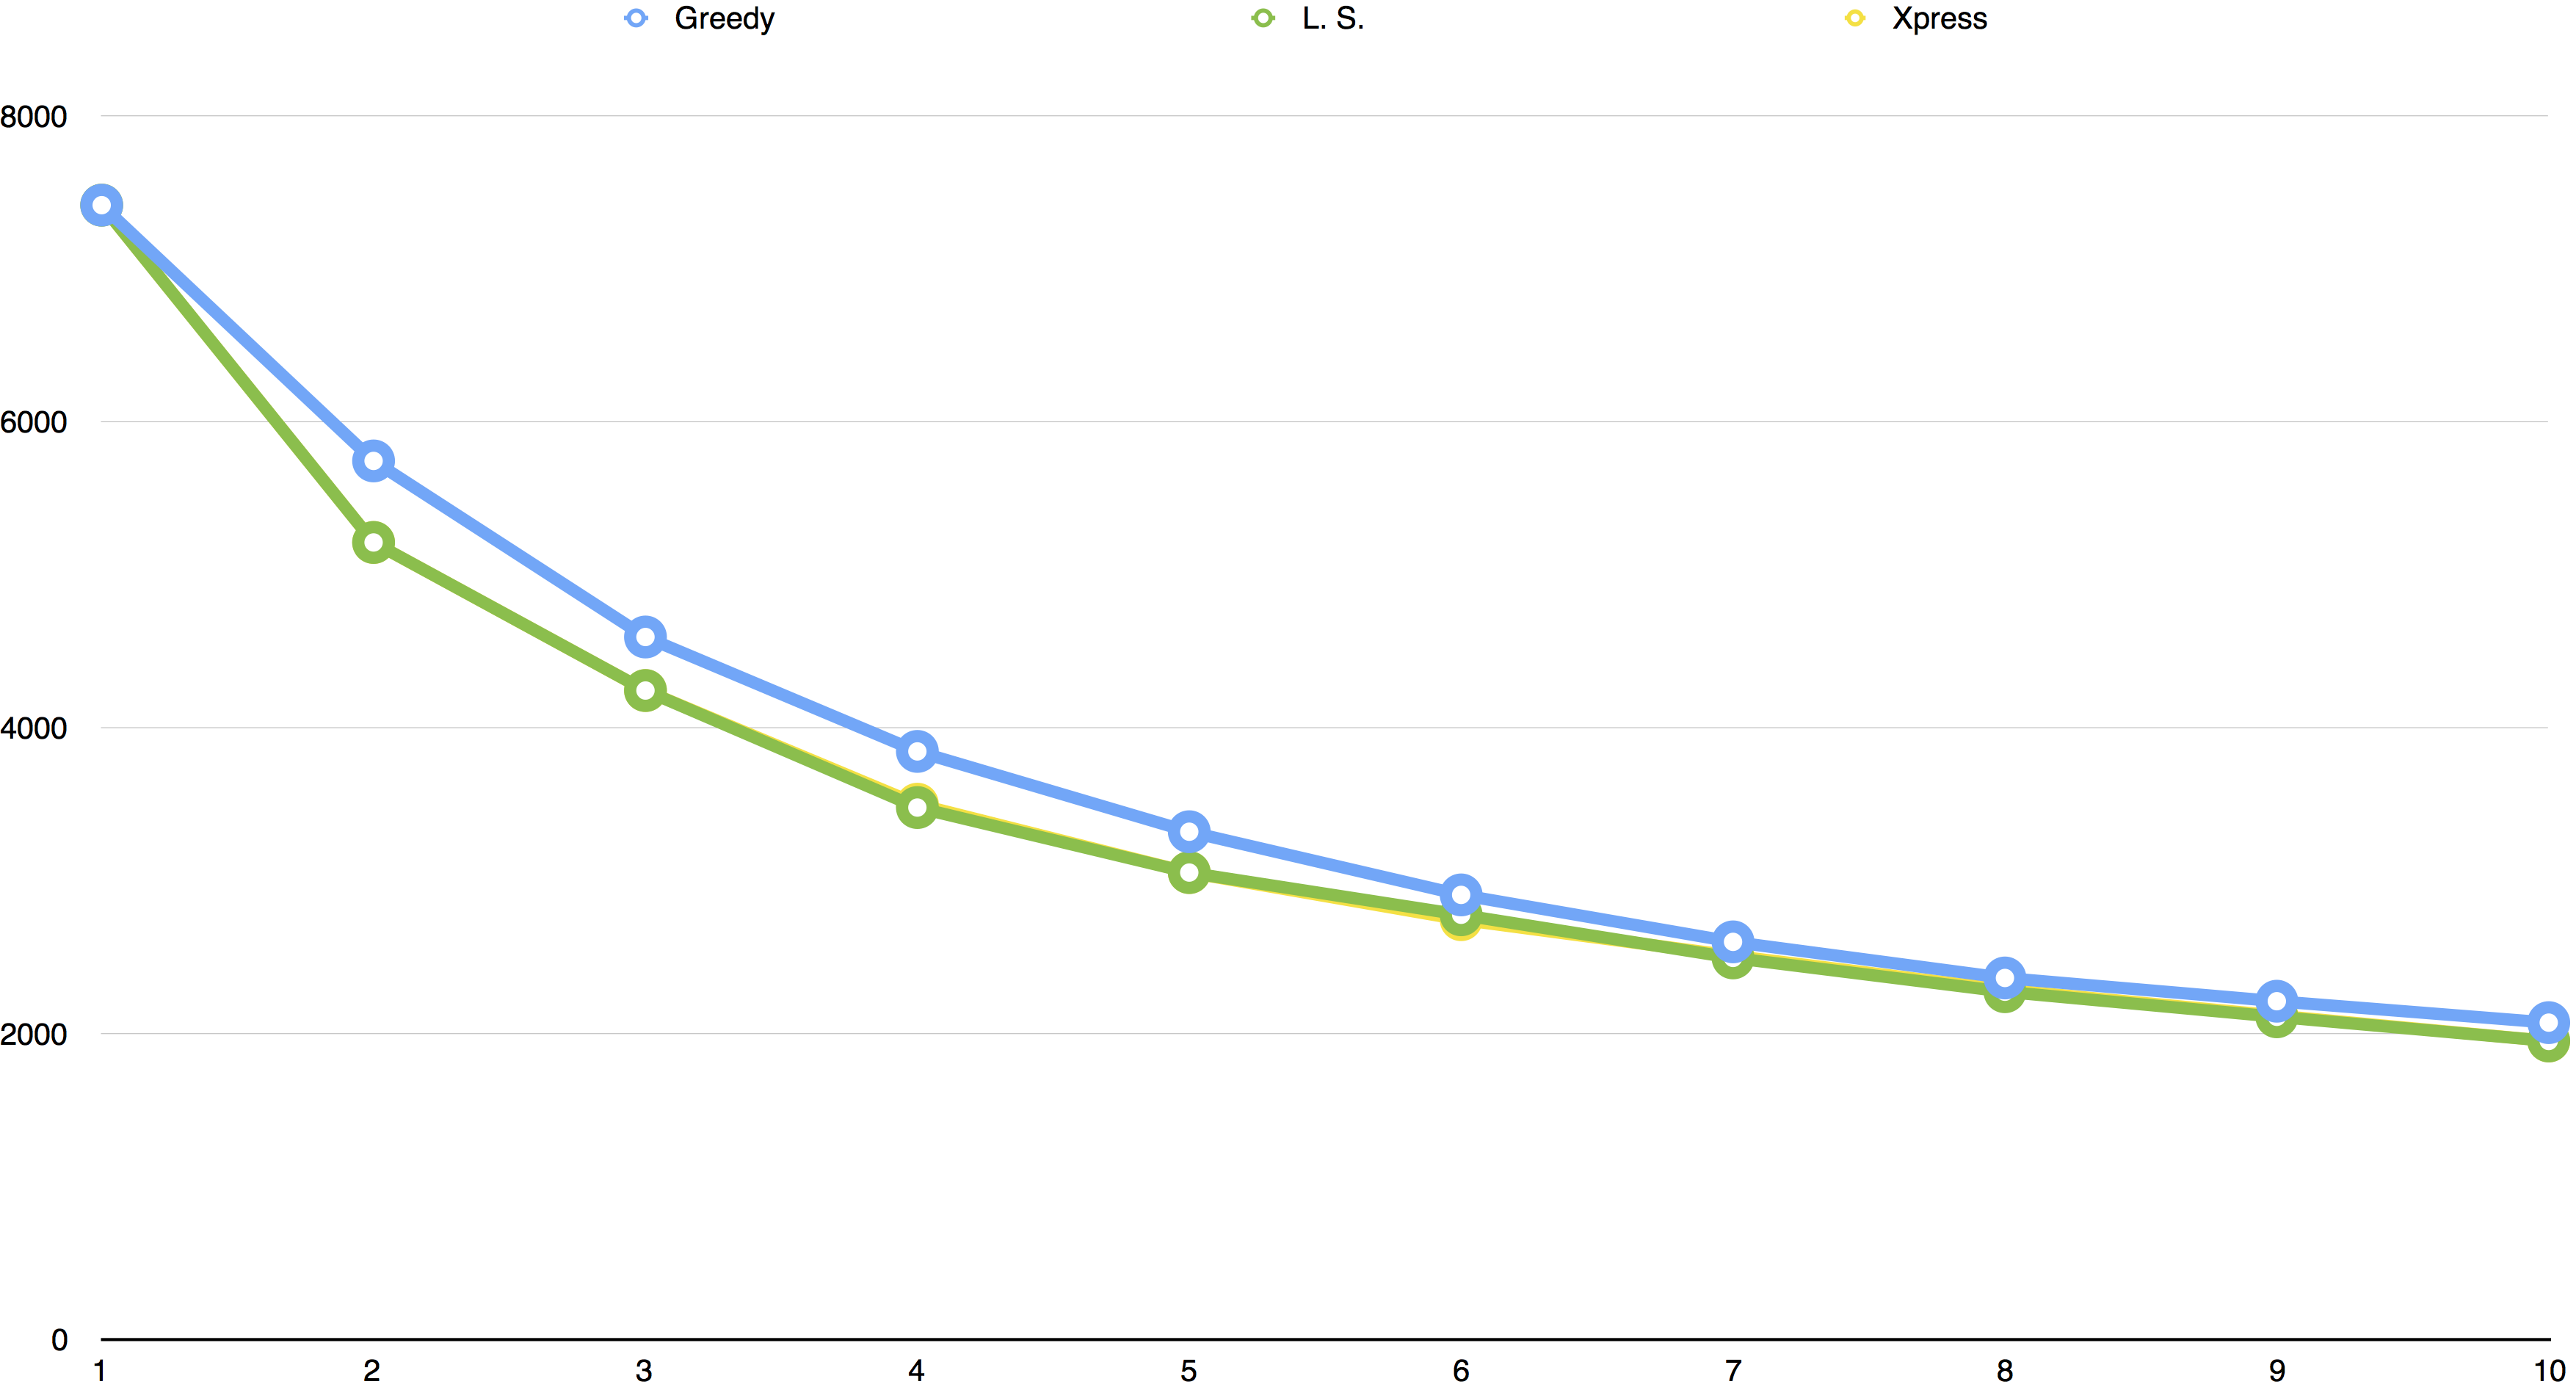
\includegraphics[width=0.8\textwidth]{tema-3-p8-c}
				\end{center}
				\caption{Resultados del problema \emph{P-Median} aplicado a los datos de \emph{100 poblaciones}}
				\label{fig:sol-8c}
			\end{figure}

			\begin{figure}[h]
				\begin{center}
					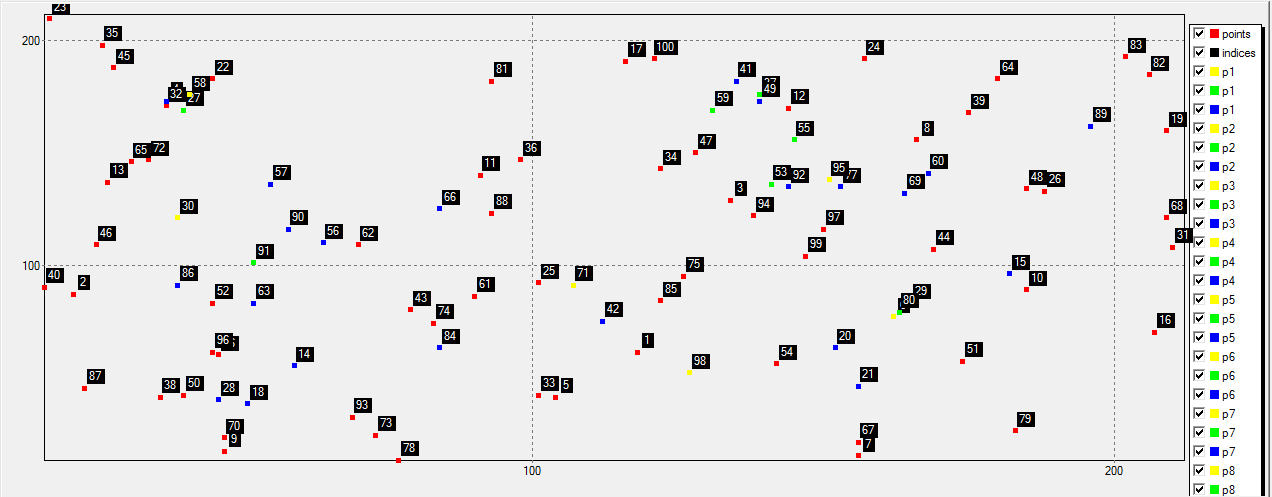
\includegraphics[width=0.8\textwidth]{tema-3-p8-c-graph}
				\end{center}
				\caption{Representación gráfica del problema \emph{P-Median} aplicado a los datos de \emph{100 poblaciones}}
				\label{fig:sol-8c-graph}
			\end{figure}

			\begin{table}[h]
				\begin{center}
					\csvautotabular{../results/csv/tema-3-p8-c.csv}
				\end{center}
				\caption{Resultados del problema \emph{P-Median} aplicado a los datos de \emph{100 poblaciones}}
				\label{table:sol-8c}
			\end{table}

%-----------------------------
%	BIBLIOGRAPHY
%-----------------------------
	\nocite{subject:mio}
	\nocite{garciparedes:mosel-examples}
	\bibliographystyle{acm}
  \bibliography{bib/misc}

\end{document}
